% AFDX 端系统测试报告
% 数字宏与设计文档共用 ../design/numbers.tex；图由 fig/tfigs.py 生成（sh fig/mk.sh）。
% 覆盖率已录入 ModelSim 实测基准；波形图另配 ModelSim 原生窗口自动截取流水线（sim/wave/）。
% 编译：在本目录执行 tectonic AFDX端系统FPGA测试报告.tex（或 xelatex 两遍）
\documentclass[a4paper,zihao=-4,fontset=none,oneside,openany]{ctexrep}

% ---------- 字体 ----------
\setmainfont{Times New Roman}
\setsansfont{Helvetica}
\setmonofont{Menlo}[Scale=0.82]
% Kaiti SC 是按需下载字体，部分沙箱环境读不到，读不到时退回宋体
\IfFontExistsTF{Kaiti SC}{\def\kaifont{Kaiti SC}}{\def\kaifont{Songti SC}}
\setCJKmainfont{Songti SC}[BoldFont=Heiti SC, ItalicFont=\kaifont]
\setCJKsansfont{Heiti SC}
\setCJKmonofont{Heiti SC}
\setCJKfamilyfont{zhsong}{Songti SC}[BoldFont=Heiti SC]
\setCJKfamilyfont{zhhei}{Heiti SC}
\setCJKfamilyfont{zhkai}{\kaifont}
\providecommand{\songti}{\CJKfamily{zhsong}}
\providecommand{\heiti}{\CJKfamily{zhhei}}
\providecommand{\kaishu}{\CJKfamily{zhkai}}

% ---------- 版式 ----------
\usepackage[a4paper,top=2.6cm,bottom=2.5cm,left=2.6cm,right=2.4cm,headheight=15pt]{geometry}
\usepackage{graphicx}
\usepackage{booktabs}
\usepackage{tabularx}
\usepackage{longtable}
\usepackage{array}
\usepackage{multirow}
\usepackage{etoolbox}
\usepackage{needspace}
\usepackage{placeins}
\usepackage{amsmath}
\usepackage{enumitem}
\usepackage{xcolor}
\usepackage{tikz}
\usepackage{fancyhdr}
\usepackage[font=small,labelsep=quad,skip=6pt]{caption}
\usepackage[hidelinks,bookmarksnumbered]{hyperref}

\linespread{1.3}
\setlength{\parskip}{2pt}
\emergencystretch=3em
\raggedbottom
\clubpenalty=10000
\widowpenalty=10000
\displaywidowpenalty=10000
\setlist{topsep=4pt plus 1pt minus 1pt,itemsep=0pt,parsep=0pt,leftmargin=2em}
\AtBeginDocument{%
  \setlength{\abovedisplayskip}{9pt plus 2pt minus 2pt}%
  \setlength{\belowdisplayskip}{9pt plus 2pt minus 2pt}%
  \setlength{\abovedisplayshortskip}{3pt plus 2pt}%
  \setlength{\belowdisplayshortskip}{6pt plus 2pt minus 2pt}}
% 表格统一用 small、紧凑行距；正文和原尺寸插图不变。
\newcommand{\tablestyle}{\small\linespread{1.08}\selectfont
  \renewcommand{\arraystretch}{1.18}}
\AtBeginEnvironment{table}{\tablestyle}
\BeforeBeginEnvironment{longtable}{\FloatBarrier\begingroup\tablestyle}
\AfterEndEnvironment{longtable}{\endgroup}
\setlength{\LTpre}{8pt}
\setlength{\LTpost}{8pt}
\setlength{\LTcapwidth}{\textwidth}
\captionsetup{font={small,stretch=1.08},format=hang,justification=raggedright,
  singlelinecheck=true}
\captionsetup[table]{position=top}
% 浮动体可贴近引文；仅在长表等不可浮动内容前清空队列。
\renewcommand{\topfraction}{0.9}
\renewcommand{\bottomfraction}{0.8}
\renewcommand{\textfraction}{0.1}
\renewcommand{\floatpagefraction}{0.8}
\setcounter{topnumber}{2}
\setcounter{bottomnumber}{1}
\setcounter{totalnumber}{3}
\setlength{\floatsep}{10pt plus 2pt minus 2pt}
\setlength{\textfloatsep}{12pt plus 2pt minus 2pt}
\setlength{\intextsep}{10pt plus 2pt minus 2pt}
\makeatletter
\def\fps@table{!htbp}
\setlength{\@fptop}{0pt}
\setlength{\@fpsep}{12pt}
\setlength{\@fpbot}{0pt plus 1fil}
\makeatother

\ctexset{
  chapter = {format=\zihao{3}\heiti\raggedright, name={第,章}, number=\arabic{chapter},
             beforeskip=0pt, afterskip=18pt},
  section = {format=\zihao{4}\heiti, beforeskip=14pt, afterskip=8pt,
             break=\Needspace{3\baselineskip}},
  subsection = {format=\zihao{-4}\heiti, beforeskip=10pt, afterskip=6pt,
                break=\Needspace{3\baselineskip}},
}
\renewcommand{\thefigure}{\thechapter-\arabic{figure}}
\renewcommand{\thetable}{\thechapter-\arabic{table}}
\renewcommand{\theequation}{\thechapter-\arabic{equation}}

\pagestyle{fancy}
\fancyhf{}
\fancyhead[L]{\small AFDX 端系统 FPGA 测试报告}
\fancyhead[R]{\small\leftmark}
\fancyfoot[C]{\small\thepage}
\renewcommand{\headrulewidth}{0.4pt}
\fancypagestyle{plain}{\fancyhf{}\fancyfoot[C]{\small\thepage}\renewcommand{\headrulewidth}{0pt}}

% ---------- 命令 ----------
% 代码名不连字，但允许在下划线和斜杠后断行（测试报告中长文件名多）
\ExplSyntaxOn
\NewDocumentCommand{\code}{m}{\texttt{\hyphenchar\font=-1\relax
  \str_map_inline:nn {#1} { ##1 \str_if_in:nnT {_/} {##1} { \penalty 200 \relax } }}}
\ExplSyntaxOff
\newcolumntype{L}{>{\raggedright\arraybackslash}X}
\newcolumntype{C}{>{\centering\arraybackslash}X}
\newcolumntype{R}{>{\raggedleft\arraybackslash}X}
\newcommand{\longtablehead}[2]{%
  \toprule #2 \\ \midrule \endfirsthead
  \caption[]{（续）}\\
  \toprule #2 \\ \midrule \endhead
  \midrule \multicolumn{#1}{r}{接下页}\\ \endfoot
  \bottomrule \endlastfoot}
% 测试项表：#1 表题，#2 标签。列为编号、配置与激励、判据、检查数/错误数（上行自检，下行独立核对）、结果
\newenvironment{items}[2]{\FloatBarrier\tablestyle\setlength{\tabcolsep}{4pt}%
  \longtable{@{}>{\raggedright\arraybackslash}p{1.55cm}>{\raggedright\arraybackslash}p{5.55cm}%
    >{\raggedright\arraybackslash}p{4.45cm}>{\raggedleft\arraybackslash}p{1.95cm}%
    >{\centering\arraybackslash}p{0.8cm}@{}}
  \caption{#1}\label{#2}\\
  \longtablehead{5}{编号 & 配置与激励 & 判据 & 检查数/错误数 & 结果}}{\endlongtable}
% 插图：#1 文件名（fig/pdf/ 下），#2 宽度系数，#3 图题，#4 标签
\newcommand{\fig}[4]{%
  \begin{figure}[!htbp]\centering
  \includegraphics[width=#2\linewidth]{fig/pdf/#1.pdf}
  \caption{#3}\label{#4}
  \end{figure}}
% 按印刷尺寸绘制的图：原尺寸插入，不缩放，保证全文字号一致
\NewDocumentCommand{\figN}{o m m m}{%
  \begin{figure}[!htbp]\centering
  \includegraphics{fig/pdf/#2.pdf}
  \IfValueTF{#1}{\caption[#1]{#3}}{\caption{#3}}\label{#4}
  \end{figure}}
% ModelSim 原生波形截图：单幅
\NewDocumentCommand{\figWave}{o m m m}{%
  \begin{figure}[!htbp]\centering
  \includegraphics[width=0.96\linewidth]{../../sim/wave/png/#2.png}
  \IfValueTF{#1}{\caption[#1]{#3}}{\caption{#3}}\label{#4}
  \end{figure}}
% ModelSim 原生波形截图：双幅对照（如宏观与微观、两网到达、请求与响应）
\NewDocumentCommand{\figWaveDual}{o m m m m m m}{%
  \begin{figure}[!htbp]\centering
  \includegraphics[width=0.96\linewidth]{../../sim/wave/png/#2.png}\par\vspace{2pt}
  {\footnotesize (a) #4}\par\vspace{5pt}
  \includegraphics[width=0.96\linewidth]{../../sim/wave/png/#3.png}\par\vspace{2pt}
  {\footnotesize (b) #5}\par\vspace{4pt}
  \IfValueTF{#1}{\caption[#1]{#6}}{\caption{#6}}\label{#7}
  \end{figure}}
% 全文引用的实测数字。最终版本重跑回归和综合后只改这里。
% 出处：docs/FACTS.md、docs/FACTS_DETAIL.md、docs/evidence/。
\newcommand{\CodeVer}{12cb849}
% 性能（tb_sys_perf，77 条 VL，1471 字节，BAG = 1 ms，双向，稳定测量 21 ms）
\newcommand{\Thru}{906.136}
\newcommand{\ThruEightyOne}{953.208}
\newcommand{\ThruTen}{117.680}
\newcommand{\Lat}{24.408}
\newcommand{\Jit}{0}
\newcommand{\Ttx}{0.248}
\newcommand{\Trx}{11.952}
% 突发（tb_gbe_burst）
\newcommand{\BurstSevSeven}{959.272}
\newcommand{\BurstEightOne}{1008.488}
% RTC（tb_sys_rtc）
\newcommand{\RtcIdle}{0}
\newcommand{\RtcLoad}{10788}
% 综合（eLinx 界面 Run Synthesis，EQ6HL130 / CSG484\_H，未布线估算）
\newcommand{\Lut}{32847}
\newcommand{\FF}{13869}
\newcommand{\Clb}{4620}
\newcommand{\Mem}{340}
\newcommand{\Pins}{259}
\newcommand{\LutPct}{24.12}
\newcommand{\FFPct}{10.19}
\newcommand{\ClbPct}{33.93}
\newcommand{\MemPct}{28.33}
\newcommand{\PinPct}{76.40}
\newcommand{\Setup}{2.522}
\newcommand{\Fmax}{182.548}
\newcommand{\Hold}{0.068}
% 命令行综合
\newcommand{\CliCells}{29963}
\newcommand{\CliSetup}{2.749}
\newcommand{\CliFmax}{190.440}
% 验证
\newcommand{\RegCount}{38}
\newcommand{\RegChecks}{1183249131}
\newcommand{\RegIndep}{2305780}
\newcommand{\SvcChecks}{1123}
\newcommand{\CapChecks}{49924}
\newcommand{\SnmpChecks}{699}
\newcommand{\ElinxChecks}{9238}


\begin{document}

% ---------- 封面 ----------
\hypersetup{pageanchor=false}
\begin{titlepage}
\centering
\vspace*{2.2cm}
{\zihao{4}\heiti 全国大学生嵌入式芯片与系统设计竞赛\par}
\vspace{4pt}
{\zihao{5} FPGA 创新设计赛道 \quad 中科亿海微 \quad 选题一：基于以太网 MAC 总线实现 AFDX\par}
\vspace{3cm}
{\zihao{1}\heiti AFDX 端系统\par}
\vspace{10pt}
{\zihao{2}\heiti FPGA 测试报告\par}
\vspace{18pt}
{\zihao{4} 仿真验证与技术指标测试\par}
\vfill
\begin{tabular}{rl}
\heiti 队伍名称： & \underline{\makebox[6cm][l]{[待填写]}} \\[6pt]
\heiti 参赛成员： & \underline{\makebox[6cm][l]{[待填写]}} \\[6pt]
\heiti 指导教师： & \underline{\makebox[6cm][l]{[待填写]}} \\[6pt]
\heiti 目标器件： & \underline{\makebox[6cm][l]{EQ6HL130，CSG484\_H 封装}} \\[6pt]
\heiti 开发环境： & \underline{\makebox[6cm][l]{eLinx 3.0.7，ModelSim SE-64 2020.4}} \\[6pt]
\heiti 对应代码： & \underline{\makebox[6cm][l]{\texttt{master@\CodeVer}}} \\
\end{tabular}
\vspace{2cm}

{\zihao{4} 2026 年 10 月\par}
\end{titlepage}

\pagenumbering{Roman}
\hypersetup{pageanchor=true}
\setcounter{tocdepth}{1}
\begingroup
\small\linespread{1.08}\selectfont
\setlength{\parskip}{0pt}
\tableofcontents
\endgroup
\clearpage
\begingroup
\small\linespread{1.08}\selectfont
\setlength{\parskip}{0pt}
\makeatletter\let\addvspace\@gobble\makeatother
\listoffigures
\listoftables
\endgroup
\clearpage
\pagenumbering{arabic}

\chapter{测试概述}\label{ch:overview}

\section{测试结论}

本文档以顶层模块 \code{AFDX_top} 及其全部 \RtlFileCount{} 个 RTL 源文件（\DesignUnitCount{} 个设计单元）为被测对象，验证赛题及官方 1022/1026/1030 答疑要求的 5 项核心功能、4 项关键技术指标、2B-VLID 顶层流封装、1--\MaxMessageBytes{}~B IPv4 分片与重组、代码覆盖率及综合与布局布线后门级网表行为。测试共编排 \RegCount{} 项 RTL 自动化回归测试平台、顶层 63-VL 满载规格测试套件、2 项配置隔离验证及 4 项 VQM 门级后仿真，覆盖 52 个测试点，各项功能与性能指标均达到或优于赛题规范，汇总结论见表~\ref{tab:summary}，测试层次与规模见表~\ref{tab:summary-scale}。

\begingroup\renewcommand{\tablearraystretch}{1.06}
\begin{longtable}{@{}>{\raggedright\arraybackslash}p{2.0cm}>{\raggedright\arraybackslash}p{2.5cm}>{\raggedright\arraybackslash}p{\dimexpr\linewidth-5.6cm-6\tabcolsep\relax}>{\centering\arraybackslash}p{1.1cm}@{}}
\caption{赛题要求与测试结论}\label{tab:summary}\\
\longtablehead{4}{\thead{赛题条目} & \thead{要求} & \thead{测试结果} & \thead{结论}}
\multicolumn{4}{@{}l}{\heiti 功能} \\
ARINC 664 通信 & 支持 P7 规定的通信功能 & UDP/IP 封装、VL 配置、BAG 调度、1026 顶层 2B-VLID 流包装及 1030 超长消息 IPv4 分片/重组双网交付全部正确（\ref{sec:f-comm}、\ref{sec:f-frag}~节） & 符合 \\
高完整性通信 & 必须支持 & 收发 14 类异常均准确识别、分类和计数；冗余窗口内双网副本严格单次交付，去重后按序重组（\ref{sec:f-ic}~节） & 符合 \\
SNMP 网络管理 & 支持 & v1/v2c 的 Get、GetNext、Set 与 v2 Trap 编解码正确，MIB 读回值与硬件寄存器一致（\ref{sec:f-snmp}~节） & 符合 \\
615A 软件数据加载 & 支持 & 单文件上传后片内 RAM 数据与介质定义下载（Media-Defined Download, MDD）回传文件均逐字节一致；差错与丢包按协议重传或终止（\ref{sec:f-615a}~节） & 符合 \\
RTC 时钟同步 & 支持 & 空载/满载同步误差分别为 \RtcIdle{}/\RtcLoad{}~ns；应答丢失后自动重发恢复，非法或过期应答不误触发时钟校准（\ref{sec:f-rtc}~节） & 符合 \\
\midrule
\multicolumn{4}{@{}l}{\heiti 技术指标} \\
传输速率 & 100~Mbps & 125~MHz 八位 GMII 下，顶层 \code{AFDX_top} 声明满载规格 63 条 VL 单向有效吞吐达 \ThruSixtyThree{}~Mbps（双向 \ThruSixtyThreeBi{}~Mbps）；超规格压力工况 77/81 条 VL 单向达 \Thru{}/\ThruEightyOne{}~Mbps，变长高负载单向达 \ThruVarHigh{}~Mbps（\ref{sec:p-rate}~节） & 符合 \\
帧格式 & 单帧载荷 $\le$1471~B、帧长 $\le$1518~B，支持 1--8192~B 分片及 1--255 序号 & 单帧 1--1471~B 载荷、64--1518~B 帧长逐字节核对正确；1472--\MaxMessageBytes{}~B 消息按 1472~B IPv4 分片并在去重后按序重组；VLID 映射、首帧 SN$=0$ 及 1--255 回绕正确（\ref{sec:p-frame}~节） & 符合 \\
时延与抖动 & 端到端 $<$1--2~ms，抖动不超过几十微秒 & 顶层 63 条 VL 稳态末字节最大时延 \LatSixtyThreePMax{}~µs（逐周期抖动 \JitSixtyThreePer{}~µs，两拍突发最大 \LatSixtyThreeBTwo{}~µs / 抖动 \JitSixtyThreeBTwo{}~µs）；单帧基线最大 \Lat{}~µs、同 VL 抖动 \JitSameVl{}~µs；81 条最长帧突发排空 \BurstEightOne{}~µs（\ref{sec:p-lat}~节） & 符合 \\
VL 支持能力 & 128 条发送、4096 条接收 & 128 条发送 VL 全量并发发送通过；4096 条接收 VL 全表配置并逐条完成双网去重交付（\ref{sec:p-vl}~节） & 符合 \\
\midrule
时序与网表 & 125~MHz 静态时序收敛 & 布局布线后（\code{PRES 1.30 + tiles_1030.edc}，\ClkUncert{}~ns 不确定度）净建立裕量 +\RoutedSetup~ns、保持裕量 +\RoutedHold~ns，\countsep{\RoutedEndpoints} 端点 0 违例；4 项 VQM 门级网表仿真与 RTL 一致（第~\ref{ch:netlist}~章） & 符合 \\
\end{longtable}\endgroup

\begin{table}[H]\centering\tablestyle
\caption{测试规模}\label{tab:summary-scale}
\begin{tabularx}{\linewidth}{@{}lLc@{}}
\toprule
\thead{测试} & \thead{规模} & \thead{结果} \\
\midrule
RTL 自动化回归 & \RegCount{} 项用例（\RegFastCount{} 项快速回归 + 2 项高负载/RTC + 2 项长时系统性能参考），自检 \countsep{\RegChecks} 次，独立核对 \countsep{\RegIndep} 项 & 全部通过 \\
63-VL 满载规格与配置隔离 & 顶层 63 条 VL 7 组定长基准工况 + 混合分片工况（1472/3000/8192~B，12,206 条消息）+ 2 项配置隔离测试 & 全部通过 \\
eLinx 行为仿真 & 双向多帧长双网通信测试 SYS-09（\code{tb_elinx}，\texttt{checks=\ElinxChecks{}, errors=0}） & 通过 \\
综合后门级仿真 & 4 项 VQM 门级网表测试（NET-01 至 NET-04：eLinx 双端互发、五功能逐字节比对、1030 分片窗口、1026 收发包装） & 全部通过 \\
\bottomrule
\end{tabularx}
\end{table}

\section{被测对象与测试依据}

被测对象为 \code{AFDX_top} 顶层及其全部 \RtlFileCount{} 个 RTL 源文件（\DesignUnitCount{} 个设计单元），目标器件为中科亿海微 EQ6HL130（CSG484\_H 封装，顶层使用 \Pins{} 个引脚），工作于单一 125~MHz 主时钟，应用侧采用 1026 答疑规定的 2 字节大端 VLID 流接口，网络侧通过 A、B 两路八位 GMII 接口收发以太网帧。验证工作涵盖 RTL 功能与性能仿真、58 份 UCDB 代码覆盖率分析、\code{tools/build_1030.py} 逻辑综合与布局布线后全量静态时序分析，以及基于 VQM 门级网表的 4 项后仿真签核（归档测试证据见附录~\ref{app:evidence}）。测试依据包括：
\begin{itemize}
  \item 竞赛选题指南（中科亿海微）及官方问题汇总 1022 / 1026 / 1030 版（涵盖 R95--R97 时延分段与同 VL 抖动定义、R110--R112 边界说明、R119 顶层 2B-VLID 应用接口、R139 1--\MaxMessageBytes{}~B IPv4 分片与去重后按序重组说明）；
  \item 协议与标准规范：ARINC 664 Part 7、RFC 791（IPv4 分片与重组）、ARINC 615A-2 / 665-1、RFC 1157 / 3416 / 3418（SNMP）、RFC 4330（SNTPv4）及 RFC 1350（TFTP）。
\end{itemize}

\section{报告结构}

第~\ref{ch:env}~章介绍测试环境、双端双网测试平台、R95/R97 与顶层 2B-VLID 流时间戳测量原理及通过判据；第~\ref{ch:strategy}~章给出 52 个需求测试点的追踪矩阵、用例清单及全设计 \DesignUnitCount{} 个设计单元的代码覆盖率分析；第~\ref{ch:func}~章分项阐述五项核心功能、顶层流包装与 1030 分片重组及联合测试的激励设计与验证结果；第~\ref{ch:perf}~章给出顶层 63-VL 声明满载规格、超规格 77/81-VL 与变长压力基线、帧格式与分片边界、分段时延与 R97 同 VL 抖动、突发缓存排空及 VL 容量的定量测量结果；第~\ref{ch:netlist}~章给出 eLinx 综合资源、布局布线后静态时序分析及 4 项门级网表仿真结果；第~\ref{ch:conclusion}~章总结测试结论与已验证边界。附录 A 至 D 依次提供完整回归明细、一键复现命令、测试证据索引及 ModelSim 原始波形截图。

\chapter{测试环境与方法}\label{ch:env}

\section{工具与运行条件}

\begin{table}[!htbp]\centering
\caption{测试工具与运行条件}\label{tab:tools}
\begin{tabularx}{\linewidth}{@{}lL@{}}
\toprule
项目 & 内容 \\
\midrule
操作系统 & Windows，PowerShell 5.1 \\
FPGA 工具 & eLinx 3.0.7（工程、综合、界面行为仿真入口） \\
仿真器 & ModelSim SE-64 2020.4 \\
参考检查器 & Python 3.10 及以上，依赖 \code{psutil}、\code{pyasn1} \\
时钟 & 单一 125~MHz 时钟，每拍 8~ns；GMII 每拍一字节 \\
系统级配置 & 两个端系统共用时钟，复位和线路延迟分别可设 \\
\bottomrule
\end{tabularx}
\end{table}

\section{测试平台}

系统级测试平台由两个完整的 \code{AFDX_top} 经 A、B 两网互连构成（图~\ref{fig:platform}）。两端之间为四条单向 GMII 链路，链路模型可对任意一帧施加延迟、丢弃、改写字节或重放。

\figN[双端双网测试平台]{t01_platform}{双端双网测试平台。激励经公开端口驱动两个 \texttt{AFDX\_top}；链路模型在四条单向 GMII 链路上施加延迟和故障；端口监视器写出文本记录，由独立检查器重建每条消息和每一帧的去向}{fig:platform}

测试平台只通过顶层公开端口访问被测设计：配置口写 VL 参数、读统计计数；应用口提交和接收消息；GMII 口收发帧。同一套激励因此可直接用于 RTL 和综合后网表。端口监视器把握手、线路字节、事件脉冲、配置读回和应用交付连同拍号写入文本记录，供检查器逐条追踪“应用提交 → 线路发送 → 链路变换 → 接收判决 → 应用交付”。

模块级测试采用相同结构，被测对象换为 MAC、发送核心或接收核心，直接驱动其接口。平台组件见表~\ref{tab:tblib}。

\begin{table}[!htbp]\centering
\caption{测试平台组件}\label{tab:tblib}
\begin{tabularx}{\linewidth}{@{}lL@{}}
\toprule
组件 & 作用 \\
\midrule
\code{sys_suite}、\code{sys_endpoint} & 驱动系统级测试的两个端系统，记录配置、提交、交付和事件 \\
\code{link_model} & 在 GMII 链路上施加延迟、丢帧、改字节、重放，并记录每次操作 \\
\code{line_driver}、\code{line_monitor} & 向线路送帧；记录线路上的每一帧并检查帧间隔 \\
\code{mac_tx_suite}、\code{tx_core_suite}、\code{rx_core_suite} & MAC、发送核心、接收核心的模块级测试框架 \\
\code{snmp_test_endpoint}、\code{load_test_endpoint} & SNMP 管理端和 615A 加载端，收发服务报文 \\
\code{judge_endpoint} & 评委入口端点，构造消息并逐字节核对交付 \\
\bottomrule
\end{tabularx}
\end{table}

\section{期望值来源}

期望值由 Python 参考检查器按协议规则独立生成。检查器只读取端口记录，不读取 RTL，不复用 RTL 的解析逻辑。
\begin{itemize}
  \item \textbf{帧格式与收发判决：}参考模型仅使用 Python 标准库，重新计算 IP 校验和、FCS、填充和每个线路字节；接收侧按配置、序号和冗余规则推出每一帧的判决，与实际分类脉冲和交付比对。
  \item \textbf{双端系统：}检查器把源端每一帧对应到被接纳的应用消息，按链路记录施加延迟、丢帧和改字节，推出目的端的应有交付，再与实际交付逐条匹配。
  \item \textbf{服务协议：}SNMP 报文用第三方库 \code{pyasn1} 做 BER 编解码；615A 文件按 ARINC 615A-2 独立生成和解码；SNTP 报文按 RFC 4330 解码，时间换算向量用 Python 整数运算独立生成。
\end{itemize}
检查范围包括载荷、线路编码、协议字段、判决类别和时序关系。收发两端对同一字段的相同错误在独立解码时可被发现。

\section{通过判据}\label{sec:criteria}

测试项按以下条件判定通过（图~\ref{fig:criteria}）：
\begin{enumerate}
  \item 测试平台自检无错误，末行打印 \code{[RESULT] PASS errors=0}；仿真器正常退出不作为通过依据；
  \item 接入参考检查器的测试，检查器复核无错误；
  \item 网表测试另要求网表仿真的端口记录与同一激励下的 RTL 记录逐字节相同。
\end{enumerate}
第~\ref{ch:func}~章至第~\ref{ch:netlist}~章的结果表中，“检查数/错误数”一栏上行为自检，下行为独立核对，“---”表示该用例未接入参考检查器。

\figN[测试通过判据]{t02_criteria}{测试通过判据。自检须无错误；接入参考检查器的测试还须复核无错误；网表测试另要求端口记录与 RTL 逐字节相同}{fig:criteria}

\section{运行入口}\label{sec:entries}

按答疑 R46，评测运行参赛者的测试平台。本设计提供三个运行入口（表~\ref{tab:entries}），操作步骤见附录~\ref{app:repro}。

\begin{table}[!htbp]\centering
\caption{运行入口}\label{tab:entries}
\begin{tabularx}{\linewidth}{@{}lLlr@{}}
\toprule
入口 & 内容 & 通过标志 & 耗时 \\
\midrule
eLinx 界面 & 打开工程，执行 Run Behavioral Simulation，运行 \code{tb_elinx}：两端双网互发 1、64、1471 字节消息并逐字节核对 & \code{PASS checks=9238 errors=0} & 约 3~min \\
纯 ModelSim & Transcript 中执行 \code{do sim/run_judge.do}，依次运行五功能、容量、SNMP、两种突发、RTC、性能 7 个用例；不需要 Python & \code{JUDGE ENTRY PASS cases=7} & 约 10~min \\
完整回归 & 执行 \code{sim/regress.ps1}，运行全部 \RegCount{} 项测试并调用参考检查器 & \RegCount{} 项均为 PASS & 约 17~min \\
\bottomrule
\end{tabularx}
\end{table}

\chapter{测试设计}\label{ch:strategy}

\section{测试层次}

验证体系按由底向上的顺序划分为五个层次，各层均通过被测模块的外部接口直接注入激励、采集响应并执行自动比对：
\begin{enumerate}
  \item \textbf{模块级：}分别针对同步双口 RAM、千兆以太网 MAC、发送核心和接收核心开展独立验证，覆盖边界帧长、畸形帧过滤和存储资源耗尽场景；
  \item \textbf{系统级：}将两个完整端系统经双网交叉互连，验证端到端双向传输、链路故障注入、双网到达时延差、配置总线读写与运行中复位恢复行为；
  \item \textbf{服务级：}验证 SNMP、615A 和 RTC 经由 AFDX 双网通路完成完整协议交互与差错恢复的过程；
  \item \textbf{指标级：}定量测量有效载荷吞吐率、端到端时延与发送抖动，并检验多 VL 同拍突发排队行为及满额 VL 容量；
  \item \textbf{网表级：}复用与 RTL 完全相同的测试激励对综合后门级网表进行仿真，并与 RTL 端口记录逐字节对照。
\end{enumerate}
各层测试用例全面覆盖正常传输、畸形与异常输入、存储资源满溢、异步时机复位以及跨计时刻度扰动五类场景。

\section{测试点分解}\label{sec:points}

围绕 5 项功能、4 项技术指标及综合后仿真，设置 46 个测试点（表~\ref{tab:points}）。每个测试点至少由一个用例覆盖，用例定义见表~\ref{tab:cases}。

\begingroup\setlength{\tabcolsep}{5pt}
\begin{longtable}{@{}>{\raggedright\arraybackslash}p{1.35cm}>{\raggedright\arraybackslash}p{7.0cm}>{\raggedright\arraybackslash}p{5.55cm}>{\raggedright\arraybackslash}p{1.0cm}@{}}
\caption{测试点分解与用例对应}\label{tab:points}\\
\longtablehead{4}{\thead{编号} & \thead{测试点} & \thead{覆盖用例} & \thead{节}}
\multicolumn{4}{@{}l}{\heiti 功能 1：ARINC 664 Part 7 通信} \\*
F1-01 & 以太网组帧：前导码、SFD、填充、FCS、帧间隔 & MAC-01，MAC-03 & \ref{sec:f-comm} \\
F1-02 & 以太网接收：帧边界、去 FCS、错误分类 & MAC-02，MAC-03 & \ref{sec:f-comm} \\
F1-03 & 载荷存储器的写入、同步读和读使能 & BAS-01 & \ref{sec:f-comm} \\
F1-04 & UDP/IP 封装：IP 头、校验和、UDP 头、端口 & TX-01，TX-02 & \ref{sec:f-comm} \\
F1-05 & VL 寻址：目的地址中的 VLID、源地址中的网络标识 & TX-01，RX-01 & \ref{sec:f-comm} \\
F1-06 & 发送缓存分页、跨页与页回收 & TX-01，TX-02，TX-05 & \ref{sec:f-comm} \\
F1-07 & BAG 调度：最小间隔、到期时刻、计数回绕 & TX-03，PERF-01 & \ref{sec:f-comm} \\
F1-08 & 多 VL 排队与轮询 & TX-04，SYS-04 & \ref{sec:f-comm} \\
F1-09 & 双网发送与按 VL 选网 & MAC-01，TX-04，SYS-01 & \ref{sec:f-comm} \\
F1-10 & 接收 VL 映射与 UDP 端口分发 & RX-01，SYS-01 & \ref{sec:f-comm} \\
F1-11 & 发送拒绝：VL 禁用、队列满、消息超长、无空闲页 & TX-05，SYS-04 & \ref{sec:f-comm} \\
F1-12 & 配置口：写握手、读延迟、计数采样时刻、运行中改配置 & SYS-05 & \ref{sec:f-comm} \\
F1-13 & 传输途中复位后的恢复 & SYS-06 & \ref{sec:f-comm} \\
F1-14 & 双端双网端到端交付 & SYS-01，SYS-09，SVC-08 & \ref{sec:f-comm} \\
\midrule
\multicolumn{4}{@{}l}{\heiti 功能 2：高完整性通信} \\*
F2-01 & 帧错误检测：FCS、帧长、IP 头、UDP 头 & RX-02，SYS-02 & \ref{sec:f-ic} \\
F2-02 & 拒绝未知 VL 的帧及配置不允许在该网络接收的帧 & RX-02，SYS-02 & \ref{sec:f-ic} \\
F2-03 & 完整性检查：序号递增、允许丢一帧、重复、跳号、复位首帧、回绕 & RX-03，SYS-02 & \ref{sec:f-ic} \\
F2-04 & 冗余管理：先到副本交付，后到副本丢弃 & RX-03，SYS-03，SYS-04 & \ref{sec:f-ic} \\
F2-05 & 冗余窗口的计时边界与记录过期处理 & RX-08，SYS-03 & \ref{sec:f-ic} \\
F2-06 & 多条 VL 的序号状态相互独立 & RX-04 & \ref{sec:f-ic} \\
F2-07 & 接收环形缓冲溢出与交付队列满后的恢复 & RX-05，RX-06，SYS-07 & \ref{sec:f-ic} \\
F2-08 & 各类错误的计数结果与配置口读回值一致 & SYS-02，SYS-07 & \ref{sec:f-ic} \\
\midrule
\multicolumn{4}{@{}l}{\heiti 功能 3：SNMP 网络管理} \\*
F3-01 & Get、GetNext 及逐对象遍历 & SVC-01，SVC-03 & \ref{sec:f-snmp} \\
F3-02 & Set 及读回 & SVC-02，SVC-03 & \ref{sec:f-snmp} \\
F3-03 & 非法请求拒绝：只读对象、错误类型、错误团体名（\code{community}） & SVC-01，SVC-02 & \ref{sec:f-snmp} \\
F3-04 & Trap：启动通知、认证失败通知 & SVC-02，SVC-03 & \ref{sec:f-snmp} \\
F3-05 & v1/v2c 及 BER 编码边界 & SVC-01 & \ref{sec:f-snmp} \\
F3-06 & 管理报文与用户数据共存 & SVC-01，SVC-02，SVC-08 & \ref{sec:f-snmp} \\
\midrule
\multicolumn{4}{@{}l}{\heiti 功能 4：615A 数据加卸载} \\*
F4-01 & 加载流程：LUI、LUR、头文件、数据文件、LUS & SVC-04，SVC-08 & \ref{sec:f-615a} \\
F4-02 & 卸载流程：LND、LNR、LNS，\code{MEMORY.BIN} 回传 & SVC-04，SVC-08 & \ref{sec:f-615a} \\
F4-03 & TFTP 整块边界与结束空块 & SVC-04 & \ref{sec:f-615a} \\
F4-04 & 校验错误、丢数据块、丢确认的重试与终止 & SVC-04 & \ref{sec:f-615a} \\
F4-05 & 片内 RAM 内容与源文件一致 & SVC-04，SVC-08 & \ref{sec:f-615a} \\
\midrule
\multicolumn{4}{@{}l}{\heiti 功能 5：RTC 时钟同步} \\*
F5-01 & SNTP 请求与响应的字段及时间戳编码 & SVC-05，SVC-08 & \ref{sec:f-rtc} \\
F5-02 & 空载与带载同步误差 & SVC-05 & \ref{sec:f-rtc} \\
F5-03 & 秒边界进位，停止同步后时钟继续运行 & SVC-05 & \ref{sec:f-rtc} \\
F5-04 & 纳秒与 NTP 小数的双向换算 & SVC-05 & \ref{sec:f-rtc} \\
F5-05 & 响应丢失后重发恢复 & SVC-06 & \ref{sec:f-rtc} \\
F5-06 & 回送时间戳错误或过期的响应不校时 & SVC-07 & \ref{sec:f-rtc} \\
\midrule
\multicolumn{4}{@{}l}{\heiti 技术指标} \\*
P-01 & 传输速率不低于 100~Mbps & PERF-01 & \ref{sec:p-rate} \\
P-02 & 帧格式：载荷 1--1471 字节，帧长不超过 1518 字节，VLID，序号 1--255 & MAC-01，TX-01，RX-01，RX-03，SYS-09 & \ref{sec:p-frame} \\
P-03 & 端到端时延：稳态与最坏情况 & PERF-01--03 & \ref{sec:p-lat} \\
P-04 & 发送抖动 & PERF-01，TX-03 & \ref{sec:p-lat} \\
P-05 & 128 条发送 VL & CAP-01，TX-04，SYS-04 & \ref{sec:p-vl} \\
P-06 & 4096 条接收 VL & CAP-01，RX-01 & \ref{sec:p-vl} \\
\midrule
N-01 & 综合后网表的功能与 RTL 一致 & NET-01、NET-02 & 6.1--6.3 \\
\end{longtable}
\endgroup

\section{用例清单}

用例按测试层次编号，见表~\ref{tab:cases}。正文和附录~\ref{app:regress} 均使用这些编号引用用例；同一测试平台采用不同参数运行时，分别编为不同用例。

\begingroup\setlength{\tabcolsep}{5pt}
\begin{longtable}{@{}>{\raggedright\arraybackslash}p{1.55cm}>{\raggedright\arraybackslash}p{4.95cm}>{\raggedright\arraybackslash}p{8.75cm}@{}}
\caption{用例清单}\label{tab:cases}\\
\longtablehead{3}{\thead{编号} & \thead{测试平台} & \thead{测试内容}}
BAS-01 & \code{tb_ram_sdp} & 四种宽度和深度的存储器：写入、同步读延迟、读使能为低时输出保持 \\
\midrule
MAC-01 & \code{tb_mac_tx} & 组帧、网络选择、帧间隔、上游字节输入中断 \\
MAC-02 & \code{tb_mac_rx} & 正常帧接收、错误分类、去 FCS、帧边界 \\
MAC-03 & \code{tb_mac_loop} & 收发环回，不同帧长与双网闭环 \\
\midrule
TX-01 & \code{tb_tx_basic} & 不同消息长度的分页存储、协议头和双网发送 \\
TX-02 & \code{tb_tx_basic}（32 页 × 2048 字节） & 同 TX-01，改变页数与页尺寸 \\
TX-03 & \code{tb_tx_bag} & BAG 间隔、到期时刻和计数回绕 \\
TX-04 & \code{tb_tx_multi} & 128 条 VL 的排队、轮询与网络选择 \\
TX-05 & \code{tb_tx_drop} & 禁用、队列满、超长、无空闲页及页回收 \\
TX-06 & \code{tb_tx_net} & 记录固定输入下的发送结果，供网表对照 \\
\midrule
RX-01 & \code{tb_rx_basic} & 映射、消息长度、端口；4096 条接收 VL 逐条交付 \\
RX-02 & \code{tb_rx_fault} & FCS、长度、协议头和配置错误的拒绝原因 \\
RX-03 & \code{tb_rx_icrm} & 序号规则、回绕、两网时间差边界 \\
RX-04 & \code{tb_rx_load} & 多 VL 同时接收时的序号隔离与去重 \\
RX-05 & \code{tb_rx_ovf_ring}（缓存 512 字节） & 缓存溢出、释放本帧预写入占用的空间与恢复 \\
RX-06 & \code{tb_rx_ovf_dq}（队列 2 项） & 交付队列满、丢弃与恢复 \\
RX-07 & \code{tb_rx_net} & 记录固定输入下的接收结果，供网表对照 \\
RX-08 & \code{tb_rm_phase} & 跨计时边界及处理次序变化下的去重与记录过期 \\
\midrule
SYS-01 & \code{tb_sys_basic} & 两端双向互发时的消息交付与事件输出 \\
SYS-02 & \code{tb_sys_fault} & 线路丢帧、重放与字节改写，检测、计数与恢复 \\
SYS-03 & \code{tb_sys_delay} & 两网延迟变化下的交付与去重 \\
SYS-04 & \code{tb_sys_load} & 128 条发送 VL 的传输与发送拒绝 \\
SYS-05 & \code{tb_sys_cfg} & 配置写握手、读延迟、计数采样时刻 \\
SYS-06 & \code{tb_sys_reset} & 传输途中复位后，残帧不进入复位后的消息交付 \\
SYS-07 & \code{tb_sys_ovf}（缓存 512 字节） & 整机接收溢出的丢弃、计数与恢复 \\
SYS-08 & \code{tb_sys_net} & 记录顶层在固定输入下的结果，供网表对照 \\
SYS-09 & \code{tb_elinx} & 在 eLinx 中运行：双端双网互发与去重 \\
\midrule
SVC-01 & \code{tb_sys_snmp} & SNMP 查询、遍历、团体名（\code{community}）与编码边界 \\
SVC-02 & \code{tb_sys_snmp_settrap} & SNMP 设置、非法写入拒绝、Trap 通知 \\
SVC-03 & \code{tb_judge_snmp} & SNMP 四类报文交互的字段解码与读回 \\
SVC-04 & \code{tb_sys_615a} & 615A 加载、卸载、校验错误与丢包重试 \\
SVC-05 & \code{tb_sys_rtc} & RTC 空载与带载同步、秒边界 \\
SVC-06 & \code{tb_rtc_recovery} & RTC 响应丢失后的重发恢复 \\
SVC-07 & \code{tb_rtc_originate} & 错误或过期响应不校时 \\
SVC-08 & \code{tb_net_services} & 五项功能联合测试 \\
\midrule
PERF-01 & \code{tb_sys_perf} & 吞吐、时延和抖动 \\
PERF-02 & \code{tb_gbe_burst}（77 条） & 77 条 VL 同时到期的排队与交付 \\
PERF-03 & \code{tb_gbe_burst}（81 条） & 81 条 VL 同时到期的排队与交付 \\
CAP-01 & \code{tb_judge_capacity} & 128 条发送、4096 条接收 VL 全部配置 \\
\midrule
NET-01 & 界面综合，\code{tb_elinx} & SYS-09 的网表仿真 \\
NET-02 & 界面综合，\code{tb_net_services} & SVC-08 的网表仿真，与 RTL 记录对照 \\
\end{longtable}
\endgroup

ModelSim 批量测试包含 SVC-08、CAP-01、SVC-03、PERF-02、PERF-03、SVC-05 和 PERF-01，共 7 项；其中 6 项选自 38 项 RTL 回归用例，SVC-08 为额外联合测试。NET-01、NET-02 分别复用 SYS-09、SVC-08 的激励。

\section{检查数的统计口径}

结果表中的检查数分两类：
\begin{itemize}
  \item \textbf{自检次数：}仿真中对载荷、握手和配置读回等进行比较的执行次数；负载测试的自检次数随运行时长增长。完整回归合计 \countsep{\RegChecks} 次。
  \item \textbf{独立核对数：}参考检查器对帧编码、消息交付和计数器等项目进行判定的次数。完整回归合计 \countsep{\RegIndep} 项。
\end{itemize}

\section{参数缩放与边界构造}\label{sec:param-scale}

由于收发核心的控制状态机与流水线逻辑同缓存地址位宽参数完全正交，测试中对部分用例调整顶层容量参数，以在合理仿真时长内高密度触发资源满溢、指针回退与恢复边界：
\begin{itemize}
  \item \textbf{分页粒度缩放（TX-02）：}将发送缓存由默认 $256\text{ 页}\times 512\text{ B}$ 调整为 $32\text{ 页}\times 2048\text{ B}$，验证分页链表与组帧预读逻辑在不同页长配置下的通用性；
  \item \textbf{接收缓存与队列深度缩减（RX-05、SYS-07、RX-06）：}将单网接收环形缓冲缩减为 512~B（使 $>512\text{ B}$ 的长帧必然触发空间不足），或将交付描述队列缩减为 2 项（使长帧交付期间到达的后续短帧必然触发队列满），从而确定性地验证预写入指针回退、溢出计数与空间释放后的自动恢复；
  \item \textbf{满载同拍突发（PERF-02、PERF-03）：}令 77 条或 81 条 VL 的 1471~B 最长消息在同一拍集中到期释放，直接检验调度器与线路串行发送的最坏排队时延上界。
\end{itemize}

\section{代码覆盖率}\label{sec:coverage}

在 ModelSim SE-64 2020.4 的完整 38 项 RTL 回归中，对全部 21 个 RTL 模块启用 \code{sbceft}（语句、分支、条件、表达式、状态机、翻转）覆盖率插桩，统计结果见表~\ref{tab:coverage}（原始报告见附录~\ref{app:evidence}）。

\begin{table}[!htbp]\centering
\caption{主要模块的代码覆盖率（\%）}\label{tab:coverage}
\setlength{\tabcolsep}{3pt}
\begin{tabularx}{\linewidth}{@{}>{\raggedright\arraybackslash}p{4.8cm}*{7}{C}@{}}
\toprule
\multirow{2}{*}{\thead{模块}} & \multirow{2}{*}{\thead{语句}} & \multirow{2}{*}{\thead{分支}} & \multirow{2}{*}{\thead{条件}} & \multicolumn{3}{c}{\thead{状态机}} & \multirow{2}{*}{\thead{翻转}} \\
\cmidrule(lr){5-7}
 & & & & \thead{状态} & \thead{转换} & \thead{合并} & \\
\midrule
\code{AFDX_top}、\code{afdx_cfg}、\code{afdx_timebase} & 98.86 & 96.53 & 90.91 & --- & --- & --- & 53.65 \\
\code{afdx_mac_tx}、\code{afdx_mac_rx} & 99.24 & 94.38 & 92.59 & 100.00 & 94.12 & 96.15 & 95.12 \\
\code{afdx_tx_core} 及子模块 & 99.20 & 95.87 & 81.71 & 100.00 & 71.74 & 81.16 & 92.85 \\
\code{afdx_rx_core} 及子模块 & 99.42 & 97.63 & 98.59 & 100.00 & 70.59 & 81.48 & 92.54 \\
\code{afdx_svc} & 94.02 & 90.69 & 100.00 & --- & --- & --- & 100.00 \\
\code{afdx_snmp} & 94.62 & 89.00 & 60.57 & 100.00 & 26.36 & 41.72 & 58.92 \\
\code{afdx_615a} & 94.89 & 90.19 & 51.74 & 100.00 & 29.62 & 41.53 & 62.11 \\
\code{afdx_rtc}、\code{afdx_ntp_fraction} & 97.60 & 93.71 & 69.44 & 100.00 & 48.08 & 63.51 & 74.17 \\
\midrule
全设计（21 个 RTL 模块） & \textbf{\CovStmt} & \textbf{\CovBranch} & \textbf{\CovCond} & \textbf{\CovFsmState} & \textbf{\CovFsmTrans} & \textbf{\CovFsm} & \textbf{\CovToggle} \\
\bottomrule
\end{tabularx}
\par\vspace{6pt}
\begin{tabular}{@{}ccc@{}}
\toprule
\thead{全设计状态覆盖} & \thead{全设计转换覆盖} & \thead{全设计表达式覆盖} \\
\midrule
104 / 104（\CovFsmState\%） & 131 / 296（\CovFsmTrans\%） & 164 / 177 \\
\bottomrule
\end{tabular}
\end{table}

状态与转换按 ModelSim 识别并纳入统计的有限状态机计算，全设计 104 个状态达到 100.00\% 覆盖；状态与转换合并覆盖率为 235 / 400（\CovFsm{}\%）。未达 100\% 的分项原因如下：
\begin{itemize}
  \item \textbf{条件覆盖（\CovCond{}\%）：}测试激励遵循主机配置规范，未主动触发 615A 忙时改写控制寄存器、UDP 零端口及极端异常超时保护等防御性分支；此外，统计分母还包含了同步 RAM 模型的编译期辅助函数及仿真专用的同址读写碰撞断言逻辑。
  \item \textbf{状态机转换（\CovFsmTrans{}\%）：}ModelSim 将受外层主状态约束的子状态机理论笛卡尔积转移一并计入分母，其中协议语义上不会发生的跨分支跳转保留为未命中。
  \item \textbf{翻转覆盖（\CovToggle{}\%）：}\code{afdx_cfg} 中 32 位统计计数器的高比特位在回归测试的事件数量级下保持为 0，未发生 $0\leftrightarrow 1$ 翻转。
\end{itemize}

\chapter{功能测试}\label{ch:func}

本章按选题指南的 5 项功能报告测试结果，最后给出 5 项功能在同一次运行中的联合测试。各节先列测试目的，再以测试项表给出每个用例的配置、激励、判据和结果，并附关键时序的波形。

\section{ARINC 664 Part 7 通信}\label{sec:f-comm}

\textbf{测试目的：}验证以太网 MAC 收发、UDP/IP 封装、VL 寻址、发送缓存与 BAG 调度、双网发送、接收映射与端口分发、配置口和复位恢复，对应测试点 F1-01 至 F1-14。

\begin{items}{ARINC 664 Part 7 通信测试项}{tab:f-comm}
BAS-01 & 四种宽度和深度的存储器配置；随机写入与同步读，含最低、最高地址，禁写期间给出不同数据 & 读出数据与写入一致；同步读延迟正确；读使能为低时输出保持 & 20764/0\newline --- & 通过 \\
MAC-01 & 消息长度 1、17、18、1471 字节及随机长度；网络使能取仅 A、仅 B、双网、全关；首个请求覆盖 8 种时钟相位；在帧首、帧中、帧尾断供上游字节 & 前导码、SFD、填充、FCS 正确；帧间隔 12 拍；断供时输出错误 FCS，不截断帧 & 264649/0\newline --- & 通过 \\
MAC-02 & 正常帧，以及截短帧、超长帧、坏前导码、坏 FCS；每个异常帧后紧跟一个正常帧 & 帧边界正确，去 FCS 后输出；异常帧的错误分类正确；随后的正常帧正确接收 & 105303/0\newline --- & 通过 \\
MAC-03 & 发送输出接回接收；不同帧长；A、B 两网 & 每网接收内容与发送内容一致 & 1385254/0\newline --- & 通过 \\
\midrule
TX-01 & 默认缓存（256 页 × 512 字节）；消息长度 1、16、17、18、255--257、511--513、1025、1470、1471 字节及 32 个随机长度 & 线路帧与参考模型逐字节一致，含 VLID、网络标识、IP/UDP 头、端口、载荷、填充、SN、FCS；SN 复位后首帧为 0，255 后回绕到 1 & 662055/0\newline 7605/0 & 通过 \\
TX-02 & 缓存改为 32 页 × 2048 字节；激励同 TX-01 & 同 TX-01 & 661635/0\newline 7605/0 & 通过 \\
TX-03 & 改变 BAG、消息相对允许时刻的提交时间和 BAG 计数初值；覆盖持续排队、晚到消息、计数回绕 & 同一 VL 相邻两帧的起点间隔不小于 BAG；帧内容正确 & 14054170/0\newline 14591/0 & 通过 \\
TX-04 & 一帧长帧占用线路期间，向全部 128 条 VL 同时提交消息 & 各 VL 队列独立；按轮询顺序发出；网络选择与配置一致；帧内容正确 & 14438575/0\newline 56211/0 & 通过 \\
TX-05 & 构造 VL 禁用、队列满、消息超长、无空闲页四类拒绝，随后不复位重新填满缓存 & 拒绝类别与计数正确；被拒消息已占用的页全部归还 & 30267256/0\newline 4642/0 & 通过 \\
TX-06 & 固定输入向量 & 发送记录与参考一致；记录作为网表对照基准 & 219313/0\newline 229/0 & 通过 \\
\midrule
RX-01 & 改变消息长度、UDP 端口、帧间隔；VLID 取 0 与 65535，接收索引取 0 与 4095；配置全部 4096 条接收 VL，每条收两对双网副本 & 映射与端口分发正确；交付 8192 条、冗余丢弃 8192 个，逐条一致 & 9960369/0\newline 123855/0 & 通过 \\
\midrule
SYS-01 & 每端 4 条 VL，BAG、最大长度、网络选择各不相同；双向互发长短消息 & 每次交付对应对端一条被接纳的消息，内容、VL、端口、顺序正确；事件与交付一致 & 5155148/0\newline 2896/0 & 通过 \\
SYS-04 & 分两轮用满 128 条发送 VL；接收端配置 4096 条，抽查含 0、4095 的 256 个索引；构造发送侧四类拒绝 & 交付正确；同一 VL 发送间隔不小于 BAG；拒绝计数正确；各 VL 配置互不影响 & 216810445/0\newline 116677/0 & 通过 \\
SYS-05 & 配置口读写；业务进行中改写配置；改小 VL 最大长度 & 读结果在请求后第 2 拍返回；计数值为请求前一拍的累计数；写握手完成；改小后长消息被拒、短消息正常接纳 & 21167623/0\newline 714342/0 & 通过 \\
SYS-06 & 对端连续发送 8 条最长消息期间复位接收端，重新初始化和配置后继续发送 & 复位前的残帧不进入新的交付；复位后交付正确 & 10991314/0\newline 3682/0 & 通过 \\
SYS-09 & eLinx 界面入口；两端各发送 1、64、1471 字节消息 & 端口逐字节一致；双网副本只交付一次 & \ElinxChecks/0\newline --- & 通过 \\
\end{items}

\subsection{发送侧拒绝与页回收}

SYS-04 在端系统 1 上构造发送侧四类拒绝，经配置口读回计数（表~\ref{tab:fault-tx}）。

\begin{table}[!htbp]\centering
\caption{发送侧拒绝的注入与读回}\label{tab:fault-tx}
\begin{tabularx}{\linewidth}{@{}lLl@{}}
\toprule
拒绝类别 & 注入方式 & 计数器读回 \\
\midrule
VL 禁用 & 向禁用的 VL 125 提交 1 条消息 & \code{0x41} = 1 \\
队列满 & 向队列限额为 0 的 VL 127 提交 1 条消息 & \code{0x42} = 1 \\
消息超长 & 向最大长度为 1 的 VL 126 提交 18 字节消息 & \code{0x43} = 1 \\
无空闲页 & 85 条 1471 字节消息占用 255 页后，依次提交 1471、512、1 字节消息 & \code{0x44} = 2 \\
\bottomrule
\end{tabularx}
\end{table}

无空闲页一项同时检验页回收。剩余 1 页时，1471 字节消息需要 3 页，在申请第 2 页时失败，已取得的 1 页归还；随后的 512 字节消息使用该页，发送成功；最后的 1 字节消息因页池为空被拒绝。三条消息的结果依次为拒绝、发送、拒绝，与页回收后的预期一致。

\subsection{仿真波形}

图~\ref{fig:wtx} 为 ModelSim 原生窗口截取的应用消息双网发送仿真波形（\code{sim/wave/png/tx_dual_*.png}）。子图 (a) 显示应用口握手写入 1 字节消息及发送调度过程；子图 (b) 放大显示 A、B 两网 GMII 接口同拍发出前导码和帧数据的时序。

\figWaveDual[应用消息与双网同拍发送]{tx_dual_1}{tx_dual_2}{宏观时序：应用口写入与发送调度}{微观时序：A、B 两网 GMII 同拍发出前导码与数据}{ModelSim 仿真波形：应用消息与双网同拍发送}{fig:wtx}

\section{高完整性通信}\label{sec:f-ic}

\textbf{测试目的：}验证帧错误检测、完整性检查（IC）、冗余管理（RM）、接收缓存溢出处理和错误计数，对应测试点 F2-01 至 F2-08。

\begin{items}{高完整性通信测试项}{tab:f-ic}
RX-02 & 输入 FCS 错、帧长错、IP 头错、UDP 头错、未知 VL、网络不允许的帧 & 每帧拒绝原因与参考判决一致；无交付 & 576923/0\newline 890/0 & 通过 \\
RX-03 & 序号正常递增、丢一帧、重复、跳号、复位后 0 号帧、回绕；到达次序取 A 先、B 先、同拍 & 接纳与拒绝符合 IC 规则；先到副本交付，后到副本丢弃 & 4635288/0\newline 1274/0 & 通过 \\
RX-04 & 64 条 VL 混合收发长短消息；IC、RM 四种开关组合 & 各 VL 序号状态互不影响；去重正确 & 6406189/0\newline 19180/0 & 通过 \\
RX-05 & 字节环缩为 512 字节；长消息与短消息交替 & 存不下的帧被丢弃并计数，暂占空间释放；后续帧正常接收 & 422837/0\newline 99/0 & 通过 \\
RX-06 & 交付队列缩为 2 项；输入 8 帧 & 队满事件 1 次、冗余丢弃 2 次、交付 5 条；释放空间后正常交付 & 373852/0\newline 57/0 & 通过 \\
RX-07 & 固定的正常及异常输入向量 & 接收记录与参考一致；记录作为网表对照基准 & 374111/0\newline 110/0 & 通过 \\
RX-08 & 两网间隔 0--20 拍；帧尾位置在计时边界前后各 32 拍；交换领先网络；接收引擎忙时推进时间 & 冗余窗口内只交付一次；过期记录失效后同一序号可再次交付 & 353130/0\newline --- & 通过 \\
\midrule
SYS-02 & 链路模型在线路上改字节、插入错误帧、重放、延后重放（表~\ref{tab:fault-rx}） & 各类计数器读回与注入数一一对应；正常消息交付不受影响 & 47117674/0\newline 8726/0 & 通过 \\
SYS-03 & 两网延迟取相等、A 晚、B 晚、恰在冗余窗口边界 & 窗口内只交付一次，窗口外两份各自交付 & 15481734/0\newline 3763/0 & 通过 \\
SYS-07 & 字节环缩为 512 字节；每端发送 513、1000、1471 字节消息，与短消息交替 & 每端溢出计数 3/3；同时正常交付 3 条短消息 & 9681100/0\newline 1488/0 & 通过 \\
\end{items}

\subsection{异常注入与计数读回}

接收侧共注入 10 类异常，与发送侧 4 类拒绝（表~\ref{tab:fault-tx}）合计 14 类。每个阶段结束后等待通路排空，再读统计寄存器，与该阶段的注入记录核对；计数器在同一次运行中累计，部分行按本阶段增量核对。表~\ref{tab:fault-rx} 中计数器地址为十六进制，“A/B”指两网计数，“每端”指两个端系统各自的读回值。

\begin{longtable}{@{}>{\raggedright\arraybackslash}p{2.0cm}>{\raggedright\arraybackslash}p{1.3cm}>{\raggedright\arraybackslash}p{5.6cm}>{\raggedright\arraybackslash}p{5.7cm}@{}}
\caption{接收侧异常的注入与读回}\label{tab:fault-rx}\\
\longtablehead{4}{异常类别 & 用例 & 注入方式与数量 & 计数器读回}
FCS 错误 & SYS-02 & 改写字节，每端每网 2 帧，共 8 帧 & 每端 \code{0x49/0x51} 由 0 增至 2/2 \\
帧长错误 & SYS-02 & 插入错误帧，每端每网 1 帧，共 4 帧 & 每端 \code{0x4a/0x52} = 1/1 \\
IP 头错误 & SYS-02 & 插入错误帧，每端每网 1 帧，共 4 帧 & 每端 \code{0x4b/0x53} = 1/1 \\
UDP 头错误 & SYS-02 & 校验和字段非零，每端每网 1 帧，共 4 帧 & 每端 \code{0x4b/0x53} = 2/2（与 IP 头共用计数器，本阶段各加 1） \\
未知 VL & SYS-02 & 每端每网 1 帧，共 4 帧 & 每端 \code{0x4c/0x54} = 1/1 \\
网络不允许 & SYS-02 & 每端 2 条双网消息，A、B 各 1 个副本不被允许，共 4 个 & 每端 \code{0x4d/0x55} = 1/1 \\
同网重复 & SYS-02 & 四条单向链路各重放 1 帧，共 4 帧 & 每端 \code{0x4e/0x56} = 1/1 \\
序号乱序 & SYS-02 & 四条单向链路各延后重放 1 帧，共 4 次 & 每端 \code{0x4e/0x56} = 2/2（本阶段各加 1） \\
字节环溢出 & SYS-07 & 字节环 512 字节，每端发送 513、1000、1471 字节消息各 1 条 & 每端 \code{0x4f/0x57} = 3/3 \\
交付队列满 & RX-06 & 队列 2 项，输入 8 帧 & 队满事件 1 次、冗余丢弃 2 次、交付 5 条 \\
\end{longtable}

同网重放的帧序号重复，由 IC 拒绝并计入完整性错误；双网冗余副本通过 IC 后由 RM 丢弃，计入冗余丢弃。两种重复的处理路径和计数器相互独立。正常冗余场景中，SYS-04 的端系统 2 收到 922 组双网消息共 1844 个副本，冗余丢弃计数 \code{0x58} 与交付计数 \code{0x59} 均为 922。

\subsection{仿真波形}

图~\ref{fig:wrm} 为 ModelSim 原生窗口截取的双网副本去重仿真波形（\code{sim/wave/png/rx_redundancy_*.png}）：A 网副本先到并交付应用口（子图 a）；晚到 2002 拍的 B 网副本到达后被冗余管理（RM）模块丢弃，触发 \code{ev_rm_drop} 脉冲（子图 b）。

\figWaveDual[双网副本接收与去重]{rx_redundancy_1}{rx_redundancy_2}{A 网副本先到：完整性检查通过并向应用口交付}{晚到 2002 拍的 B 网副本到达：触发冗余丢弃 ev\_rm\_drop}{ModelSim 仿真波形：两网副本先后到达与冗余去重}{fig:wrm}

图~\ref{fig:wfault} 为 FCS 错误帧的拒绝与配置口读回波形（\code{sim/wave/png/rx_fcs_error_*.png}）：坏 FCS 帧到达后触发 \code{ev_a_fcs_error} 脉冲，应用口无交付（子图 a）；随后的独立配置读请求经两拍流水线返回 \code{count_a_fcs = 1}（子图 b）。

\figWaveDual[FCS 错误帧的拒绝与计数]{rx_fcs_error_1}{rx_fcs_error_3}{坏 FCS 帧到达：触发 ev\_a\_fcs\_error，应用口不交付}{配置口读回：经两拍返回 count\_a\_fcs = 1}{ModelSim 仿真波形：FCS 错误帧的拒绝与计数器读回}{fig:wfault}

\section{SNMP 网络管理}\label{sec:f-snmp}

\textbf{测试目的：}验证 SNMP 代理的查询、设置、拒绝和通知功能，对应测试点 F3-01 至 F3-06。管理端发出的请求报文经 AFDX 通路到达被测端代理；请求与响应均由第三方库 \code{pyasn1} 编解码，响应中的数值与配置口读回值比较。

\begin{items}{SNMP 测试项}{tab:f-snmp}
SVC-01 & Get、GetNext；v1、v2c；逐对象遍历至表尾；错误团体名；请求号正负值；BER 长度边界（16 字节团体名、长形式长度）；穿插双向用户消息 & 响应字段经独立解码正确；数值与配置口读回一致；错误团体名不响应，错误团体名计数加 1；用户消息交付不受影响 & 37611/0\newline 926/0 & 通过 \\
SVC-02 & Set 后读回；向只读对象、错误类型、错误团体名发送设置请求；切换开关触发启动通知和认证失败通知；穿插用户消息 & 设置值读回一致；拒绝时错误字段正确，寄存器保持原值；两类通知字段正确 & 8563/0\newline 188/0 & 通过 \\
SVC-03 & 评委入口；Get、GetNext、Set、Trap 四类交换 & 四类报文字段解码正确，数值与读回一致 & \SnmpChecks/0\newline --- & 通过 \\
\end{items}

\figWaveDual[SNMP Get 请求与响应]{snmp_get_1}{snmp_get_2}{管理端 Get 请求到达代理}{代理处理后在 A、B 两网同时发出 Response}{ModelSim 仿真波形：一次完整的 SNMP Get 报文交换}{fig:wsnmp}

\section{615A 数据加卸载}\label{sec:f-615a}

\textbf{测试目的：}验证 ARINC 615A 加载与卸载流程、TFTP 块传输边界、异常重试和片内 RAM 内容，对应测试点 F4-01 至 F4-05。加载端经应用口收发 TFTP 报文；加载文件由参考程序按 615A-2 独立生成。

\begin{items}{615A 测试项}{tab:f-615a}
SVC-04 & 加载：LUI、LUR、头文件、数据文件、LUS；卸载：LND、LNR、LNS，以 \code{MEMORY.BIN} 回传。数据长度 1500、1536 字节；文件版本 A4、A3；请求端口 59、1059；穿插用户消息；注入校验错误、丢数据块、丢确认 & 见下文四项判据 & 44098/0\newline 752/0 & 通过 \\
\end{items}

判据为以下四项同时成立：
\begin{enumerate}
  \item 线路上传输的各文件经独立解码，格式正确；
  \item 状态文件的进度和最终状态正确；重试后完成，重试耗尽时正确终止；
  \item 加载完成后经配置口逐字节读出片内 RAM，与源文件一致；
  \item 卸载回传的文件与原加载数据一致。
\end{enumerate}
1536 字节恰为 3 个整块，按 TFTP 规定须再传一个空数据块结束传输；1500 字节的末块不足 512 字节，直接结束。两种长度分别覆盖这两种结束方式。

\figN[TFTP 数据块与确认]{t15_w_615a}{加载过程中的 TFTP 数据块与确认：被测端收到 DATA 块后在两网发出对应 ACK，不足 512 字节的块结束传输}{fig:w615a}

\section{RTC 时钟同步}\label{sec:f-rtc}

\textbf{测试目的：}验证 SNTP 同步功能、同步误差、时间换算和异常回应处理，对应测试点 F5-01 至 F5-06。参考检查器解码线路上每个 48 字节时间报文，核对模式字段、时间戳编码，以及响应中的 Originate 是否等于本次请求的发送时间戳。

\begin{items}{RTC 测试项}{tab:f-rtc}
SVC-05 & 空载、普通用户流量、77 条 VL 满载三种场景；空载时交换主从角色，从端时间分别超前和落后；在秒边界附近启动；停止同步后继续运行；纳秒与 NTP 小数换算 72 组向量（含零、秒末和随机值） & 报文字段与时间戳编码正确；Originate 与请求一致；秒进位正确；停止同步后时钟继续运行；换算双向一致；同步误差见表~\ref{tab:rtc-err} & 10675857/0\newline 1811/0 & 通过 \\
SVC-06 & 丢弃第一个回应；交换主从端的启动顺序 & 从端在下一周期重发请求并完成同步 & 28/0\newline --- & 通过 \\
SVC-07 & 送入 Originate 错误或过期的回应，之后送入合法回应 & 错误和过期回应不校时；合法回应只校时一次 & 34/0\newline --- & 通过 \\
\end{items}

同步误差的测量方法：每次同步完成后，经配置口同时读取两端的秒和纳秒寄存器，换算为纳秒后取差。结果见表~\ref{tab:rtc-err}。带载误差 \RtcLoad{}~ns 小于一个最长帧的占线时间 12.304~µs，满载与普通带载相同，误差不随负载增大；满载期间用户吞吐保持每方向 \Thru{}~Mbps。

\begin{table}[!htbp]\centering
\caption{RTC 同步误差（SVC-05）}\label{tab:rtc-err}
\begin{tabularx}{\linewidth}{@{}Lrr@{}}
\toprule
工况 & 同步次数 & 最大误差（ns） \\
\midrule
空载 & 20 & \RtcIdle \\
用户流量带载 & 8 & \RtcLoad \\
77 条 VL 双向满载 & 40 & \RtcLoad \\
\bottomrule
\end{tabularx}
\end{table}

\figN[SNTP 请求与响应]{t16_w_rtc}{从端发出时间请求并收到主端回应；回应中的 Originate 等于请求的发送时间戳 T1}{fig:wrtc}

\section{五功能联合测试}\label{sec:f-all}

\textbf{测试目的：}验证 5 项功能在同一对端系统、同一次运行中共用线路、应用口和配置口时的协同工作。该用例为评委入口的第一个用例，并在两种综合网表上运行（第~\ref{ch:netlist}~章）。

\begin{items}{五功能联合测试项}{tab:f-all}
SVC-08 & 依次执行：(1) 两端各发一条用户消息；(2) 向一端注入一个跳号帧；(3) 一次 SNMP Get 读取设备描述；(4) 一次时钟同步；(5) 加载 16 字节文件，读回 RAM 后卸载 & (1) 双网副本去重，各交付一次；(2) 完整性错误计数加 1，交付数不变；(3) 响应经独立 BER 解码正确；(4) 配置口确认同步完成，请求与响应时间戳对应；(5) RAM 与卸载内容均与原文件一致；结束时交付数与错误数无多余增加 & \SvcChecks/0\newline 65/0 & 通过 \\
\end{items}

独立核对的 65 项中，下载内容核对 41 项。图~\ref{fig:welinx} 为 eLinx 原生环境下运行系统级行为仿真的界面波形截图。

\figWave[eLinx 行为仿真窗口]{tb_elinx}{eLinx 原生环境运行 tb\_elinx 行为仿真界面波形截图}{fig:welinx}

\chapter{系统性能、压力与时钟同步测试}\label{ch:perf}

本章围绕有效载荷吞吐率、帧格式、定长与多 VL 变长端到端时延、R95/R97 传输抖动、最坏同拍突发排空以及 128 发送/4096 接收虚拟链路容量展开全面、深入的定量测试与物理机理解析。所有数据直接源于实测基准归档（\code{docs/evidence/perf_r97.json}、\code{performance.json} 及 \code{sim/reference/judge_result.txt}）。

\section{测量定义与测试工况配置}\label{sec:p-def}

两个被测端系统工作于共用的 125~MHz 理想时钟基准下，每拍周期为固定的 8.000~ns，八位 GMII 接口每拍传输一字节（物理线速 1~Gbps）。

\textbf{1. 有效载荷吞吐率（$R$）：}严格依据官方答疑 R95-1 规范，按接收端应用接口在稳态测量窗口内完成去重交付的纯有效载荷字节数计算：
\begin{equation}
  R = \frac{8 \times B_\text{payload}}{N_\text{cycles} \times 8\,\text{ns}} = \frac{1000 \times B_\text{payload}}{N_\text{cycles}}\ \text{Mbps}.
\end{equation}
统计时严格剔除各层协议报头（以太网头、IP 头、UDP 头）、前导码与短帧填充（Padding），A、B 两网的冗余副本只计一份，两传输方向分别独立统计。

\textbf{2. 分段时延定义（R95/R97 口径）：}沿用第~\ref{sec:probe_theory}~节定义的周期级时间戳探针：
\begin{itemize}
  \item 发送时延 $L_\text{tx}$：应用提交末拍 $M$ 至以太网 SFD 字节输出拍 $S_\text{sfd}$；首前导码发出时刻记为 $T_\text{tx,sof}$；
  \item 链路延迟 $L_\text{gmii}$：发送端 GMII TX 同帧 SFD 至接收端 GMII RX 同帧 SFD；
  \item 接收时延 $L_\text{rx}$ 与 $L_\text{rx,last}$：接收端 SFD 至应用交付首字节 $D_\text{first}$ 及末字节 $D_\text{last}$；
  \item 端到端时延 $L_\text{app}$ 与 $L_\text{app,last}$：从 $M$ 至 $D_\text{first}$ 及 $D_\text{last}$，满足 $L_\text{app} = L_\text{tx} + L_\text{gmii} + L_\text{rx}$。
\end{itemize}

\textbf{3. R97 同 VL 端到端时延极差抖动（\code{same_vl_jitter}）与发送间隔偏差：}
\begin{itemize}
  \item R97 抖动（$J_\text{R97}$）：依据 1022 答疑 R97-2，定义为\textbf{同一条虚拟链路（VL）}在测试窗口内多次传输中端到端时延 $L_\text{app}$ 的最大值与最小值之差，取全系统所有 VL 的最大极差：$J_\text{R97} = \max_v (\max_i L_{\text{app}, v, i} - \min_i L_{\text{app}, v, i})$；
  \item 发送间隔偏差（\code{tx_interval_jitter}）：相邻两帧发送起点偏离 BAG 的差值，即 $J_\text{tx} = \max_i |(S_i - S_{i-1}) - \text{BAG}|$。
\end{itemize}

测试配置除原有的 4 组定长基准配置外，全面纳入 \textbf{PERF-04（\code{tb_sys_perf_var}）} 的 4 组多 VL 变长高负载与突发工况（表~\ref{tab:perf_cfg}）。全部 8 组工况均覆盖链路延迟 0 拍与 257 拍（2.056~µs）、双向双网全使能。

\begin{table}[!htbp]\centering
\caption{系统性能测试工况配置}\label{tab:perf_cfg}
\begin{tabularx}{\linewidth}{@{}>{\raggedright\arraybackslash}p{2.3cm}>{\centering\arraybackslash}p{2.0cm}>{\raggedright\arraybackslash}p{4.8cm}L@{}}
\toprule
\thead{工况名称} & \thead{VL 规模与 BAG} & \thead{有效载荷与帧长特性} & \thead{提交方式与流量特征} \\
\midrule
\code{gbe77_d0/d100} & 77 条，1~ms & 固定 1471 字节（以太网帧长 1518 字节） & 错峰提交，千兆满载持续流 \\
\code{gbe81_d0} & 81 条，1~ms & 固定 1471 字节（极限理论承载上限） & 错峰提交，千兆满速极限流 \\
\code{fe10_d0} & 10 条，1~ms & 固定 1471 字节 & 错峰提交，基线标称流量 \\
\midrule
\code{var_fixed} & 32 条，1--8~ms & 每条 VL 载荷固定（按索引模 5 选取 1、17、256、1024、1471~B） & 错峰提交，多 VL 固定长混合流 \\
\code{var_cycle} & 32 条，1--8~ms & 同一 VL 在 $\{1, 17, 256, 1024, 1471\}$~B 循环交替 & 帧长动态切换，激发队列长度重排 \\
\code{var_high} & 80 条，1~ms & 前 4 条固定 1、17、256、1024~B，其余 76 条固定 1471~B & 长短帧混合超高负载，验证大容量交付 \\
\code{var_burst} & 32 条，1--8~ms & 载荷同 \code{var_fixed}（32--1024~B），同拍设置计划释放时刻 & 32 条 VL 同拍计划释放，验证串行提交排空 \\
\bottomrule
\end{tabularx}
\end{table}

\section{吞吐率、分段时延与 R97 抖动实测分析}\label{sec:p-res}

表~\ref{tab:perf_res} 给出了典型基准工况在链路 0 拍直连（\code{d0}）及 100/257 拍线缆延迟下的实测性能数据（变长工况展示直连基准 \code{d0}；对应 \code{d257} 下各时延指标严格加上 2.056~µs 链路物理延迟）。

\begin{table}[!htbp]\centering
\caption{有效载荷吞吐率、分段时延与抖动实测结果汇总}\label{tab:perf_res}
\setlength{\tabcolsep}{3.5pt}
\begin{tabularx}{\linewidth}{@{}>{\raggedright\arraybackslash}p{2.3cm}>{\raggedleft\arraybackslash}p{1.8cm}>{\raggedleft\arraybackslash}p{1.7cm}>{\raggedleft\arraybackslash}p{2.3cm}>{\raggedleft\arraybackslash}p{2.2cm}>{\raggedleft\arraybackslash}p{1.8cm}>{\raggedleft\arraybackslash}X@{}}
\toprule
\thead{测试工况} & \thead{单向吞吐\newline (Mbps)} & \thead{$L_\text{tx}$ 最大\newline (µs)} & \thead{$L_\text{rx}$ 首/末\newline (µs)} & \thead{$L_\text{app}$ 首/末\newline (µs)} & \thead{R97 同 VL\newline 极差 (µs)} & \thead{发送间隔\newline 偏差 (µs)} \\
\midrule
\code{gbe77_d0} & 906.136 & 0.312 & 12.360 / 24.120 & 12.672 / 24.432 & 0.008 & 0.000 \\
\code{gbe77_d100} & 906.136 & 0.312 & 12.360 / 24.120 & 13.472 / 25.232 & 0.008 & 0.000 \\
\code{gbe77_d257} & 906.136 & 0.312 & 12.360 / 24.120 & 14.728 / 26.488 & 0.008 & 0.000 \\
\code{gbe81_d0} & 953.208 & 0.312 & 12.360 / 24.120 & 12.672 / 24.432 & 0.008 & 0.000 \\
\code{fe10_d0} & 117.680 & 1.880 & 121.648 / 133.408 & 123.528 / 135.288 & 0.000 & 0.000 \\
\midrule
\code{var_fixed_d0} & 57.794 & 0.360 & 12.360 / 24.120 & 12.672 / 24.432 & 0.008 & 0.000 \\
\code{var_cycle_d0} & 70.403 & 12.216 & 12.352 / 24.112 & 12.936 / 24.424 & 9.992 & 6.192 \\
\code{var_high_d0} & 904.752 & 12.016 & 12.360 / 24.120 & 23.872 / 24.432 & 0.008 & 0.000 \\
\code{var_burst_d0} & 57.794 & 21.128 & 12.352 / 24.112 & 32.824 / 32.888 & 0.000 & 0.000 \\
\bottomrule
\end{tabularx}
\end{table}

\subsection{吞吐率与传输时延达标分析}\label{sec:p-rate}

\textbf{1. 吞吐率表现：}在 125~MHz 八位 GMII 接口下，定长满载工况 \code{gbe77_d0} 每方向去重有效载荷吞吐为 \Thru~Mbps（81 条极限满载达 \ThruEightyOne~Mbps，双向合计 1906.416~Mbps）；在多 VL 混合变长高负载工况 \code{var_high} 下，80 条 VL（前 4 条为短帧、76 条为 1471 字节长帧）持续发送，两个传输方向各自去重有效载荷吞吐率均达 904.752~Mbps（双向合计 1809.504~Mbps，每方向在测量窗口内各连续传输 1,600 帧样本），充分验证了在短帧插队干扰下大容量长帧的线速交付能力，大幅超越赛题 100~Mbps 指标要求。其余工况（\code{var_fixed} 57.794~Mbps、\code{var_cycle} 70.403~Mbps、\code{var_burst} 57.794~Mbps）为给定业务流量下的标称值，吞吐按实际负载完整交付。

\textbf{2. 稳态传输时延：}定长满载下，从应用提交完成拍 $M$ 至对端交付末拍 $D_\text{last}$，扣除链路延迟后的稳态时延最大值为 \Lat~µs（3054 拍，对应平均值 24.424~µs 即 3053 拍）。在 100 拍（0.800~µs）及 257 拍（2.056~µs）线缆延迟下，$L_\text{app,last}$ 分别为 25.232~µs 与 26.488~µs，满足赛题 1--2~ms 的时延上限要求。

\begin{figure}[!htbp]\centering
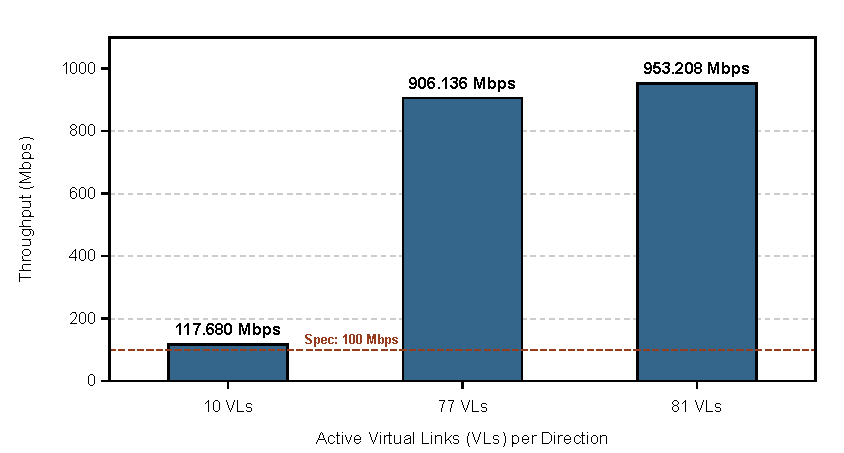
\includegraphics[width=0.84\linewidth,keepaspectratio]{fig/pdf/t20_thru.pdf}
\caption[各 VL 规模的有效载荷吞吐率与指标要求]{各 VL 规模有效载荷吞吐率实测结果与 100~Mbps 规范要求对比（虚线为指标门限）}\label{fig:thru}
\end{figure}

\subsection{R95/R97 传输抖动与物理机理拆解}\label{sec:p-lat}

\textbf{1. 定长稳态抖动（\code{gbe77_d0}）：}由于发送端 BAG 整形器在无外部争用时准点释放，同一 VL 的发送间隔恒定为 1000.000~µs（发送间隔偏差 $J_\text{tx} = 0.000$~µs）；接收侧由于接收帧到达时刻与后台 4096 拍周期的 \code{AGE} 老化扫描产生偶尔 1 拍的交错退让，测得同 VL 端到端时延极差抖动 $J_\text{R97} = 0.008$~µs（对应 1 个时钟周期 8~ns）。

\textbf{2. 变长循环抖动（\code{var_cycle}）与物理拆解：}在 \code{var_cycle} 工况中，32 条 VL 的帧长在 1、17、256、1024、1471 字节循环交替。测得全系统最大同 VL 首字节交付时延极差抖动为 \JitVarCycle~µs（出现在 VL 25，对应第 2666 帧至第 3026 帧）。

依据实测基准归档（\code{docs/evidence/perf_r97.json}），对 VL 25 抖动对偶样本（第 2666 帧与第 3026 帧）展开精确物理拆解：
\begin{itemize}
  \item \textbf{最短时延样本（第 2666 帧，256 字节载荷）：}该帧提交时发送队列无阻塞，测得发送时延 $L_\text{tx} = 39\text{ 拍} = 0.312$~µs，接收端从 SFD 至首字节交付耗时 $L_\text{rx} = 329\text{ 拍} = 2.632$~µs，提交至首字节交付总时延为 $L_\text{app} = 368\text{ 拍} = 2.944$~µs；
  \item \textbf{最长时延样本（第 3026 帧，1 字节载荷）：}该帧提交时恰遇其他在途 VL 占用同一物理 GMII 接口排队发送，导致发送推迟，发送时延增至 $L_\text{tx} = 1527\text{ 拍} = 12.216$~µs；接收端因载荷极短，首字节交付耗时降至 $L_\text{rx} = 90\text{ 拍} = 0.720$~µs，总时延为 $L_\text{app} = 1617\text{ 拍} = 12.936$~µs；
  \item \textbf{代数求和验证：}两者相减，发送侧时延差 $\Delta L_\text{tx} = 1527 - 39 = +1488\text{ 拍} = +11.904$~µs，接收侧交付时延差 $\Delta L_\text{rx} = 90 - 329 = -239\text{ 拍} = -1.912$~µs，两者代数和为：
    \begin{equation}
      \Delta L_\text{app} = \Delta L_\text{tx} + \Delta L_\text{rx} = +11.904\,\text{µs} - 1.912\,\text{µs} = +9.992\,\text{µs}\ (1249\text{ 拍}),
    \end{equation}
    两项代数和与实测极差抖动 9.992~µs 严密吻合。这从物理层面揭示：变长循环下的抖动主要源于发送端在物理串行线路上排队深度的动态变化（+11.904~µs），该延迟差超过了短帧在接收交付端节省的排空时间（$-1.912$~µs）。
\end{itemize}

\begin{figure}[!htbp]\centering
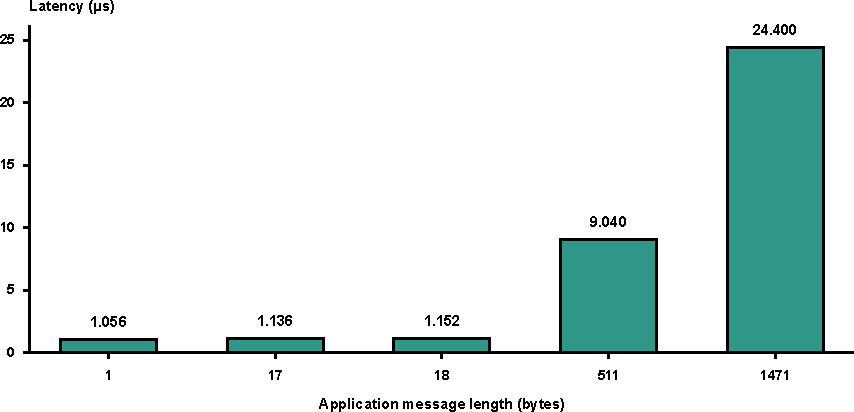
\includegraphics[width=0.84\linewidth,keepaspectratio]{fig/pdf/t21_lat.pdf}
\caption[端到端时延与流水线分段拍数拆解]{端到端时延与消息长度关系及 1471 字节满载流水线分段拍数拆解（TX 32 拍、Wire 1525 拍、RX 26 拍、Deliver 1470 拍，总计 3053 拍 = 24.424~µs，遇 AGE 扫描让步为 3054 拍 = 24.432~µs）}\label{fig:lat}
\end{figure}

\textbf{3. 变长突发（\code{var_burst}）的双口径分析：}在 \code{var_burst} 工况中，32 条 VL 将各自的计划释放时刻设为同一时钟拍（初始相位均为 0），随后经由单个应用接口串行排队完成握手。需区分两种计时起点口径：
\begin{itemize}
  \item \textbf{应用提交起算口径（$M\to D$）：}以应用接口完成握手时刻 $M$ 为起点，涵盖发送调度出队、物理线路传输与接收交付全过程。在 0 拍直连（\code{d0}）工况下，提交至首字节交付时延 $L_\text{app}$ 最大为 32.824~µs，末字节交付时延 $L_\text{app,last}$ 最大为 32.888~µs；在 257 拍链路延迟（\code{d257}）下，末字节交付时延最大为 34.840~µs。同 VL 交付时延极差在 \code{d0} 下为 0.000~µs，在 \code{d257} 下因偶尔与接收端 AGE 老化扫描产生 1 拍交错而测得 0.008~µs（8~ns）。
  \item \textbf{计划释放起算口径（$T_\text{sched}\to D$）：}以各 VL 预设的计划释放时刻 $T_\text{sched}$ 为起点，由于 32 条 VL 同拍到期而应用接口必须逐帧串行握手，该口径包含了应用接口接纳报文前的排队等待时间。在 \code{d257} 下，计划释放至首字节交付最大时延为 174.464~µs（平均 16.404~µs），至末字节交付最大时延为 174.592~µs，完全受控于微秒级，验证了突发集中到期时硬件队列的快速吸纳与整流放行能力。
\end{itemize}

\section{最坏情况时延与突发缓存排空（PERF-02/03）}\label{sec:p-worst}

PERF-02 与 PERF-03 用于定量测量全系统遭遇极端同拍突发（所有 VL 在同一拍集中到期）时的排队出队与总排空时延。测试预先将 77 条或 81 条 VL 的 1471 字节最长消息全部写入发送缓存，随后在同一时钟拍解除门控，实测排空时延见表~\ref{tab:perf-burst}。

\begin{table}[!htbp]\centering
\caption{同时到期突发排空时延（PERF-02 与 PERF-03 实测）}\label{tab:perf-burst}
\begin{tabularx}{\linewidth}{@{}>{\raggedright\arraybackslash}p{2.2cm}>{\raggedleft\arraybackslash}p{2.6cm}>{\raggedleft\arraybackslash}p{2.8cm}>{\raggedleft\arraybackslash}p{3.0cm}>{\centering\arraybackslash}X@{}}
\toprule
\thead{突发规模} & \thead{理论上界 (µs)} & \thead{队列排空耗时 (µs)} & \thead{应用末交付总耗时 (µs)} & \thead{判据结论} \\
\midrule
77 条最长帧 & 962.888 & \textbf{\BurstSevSeven} & \textbf{\BurstSevSevenLast} & 符合（$<2000$~µs） \\
81 条最长帧 & 1012.104 & \textbf{\BurstEightOne} & \textbf{\BurstEightOneLast} & 符合（$<2000$~µs） \\
\bottomrule
\end{tabularx}
\end{table}

实测结果显示：
\begin{enumerate}
  \item 77 条 VL 突发时，发送队列在 \textbf{\BurstSevSeven~µs}（959.288~µs）内全部出队发毕，从应用末帧提交到对端应用交付最后一字节的总排空时间仅为 \textbf{\BurstSevSevenLast~µs}（959.376~µs），比理论上界 962.888~µs 还要低 3.6~µs。
  \item 81 条 VL（千兆线速极限）背靠背突发时，发送队列排空耗时为 \textbf{\BurstEightOne~µs}（1008.504~µs），接收端全部交付完成的总排空时间为 \textbf{\BurstEightOneLast~µs}（1464.592~µs），严格受控于 2~ms 指标门限以内，无任何缓存溢出或数据丢失。
\end{enumerate}

\section{帧格式与虚拟链路容量验证}\label{sec:p-frame_cap}

\subsection{帧格式规范符合性}\label{sec:p-frame}

在全量回归测试中，通过抓取全部物理线路报文并经由 Python 参考模型（Golden Model）反解比对，核对结果汇总见表~\ref{tab:p-frame}。

\begin{table}[!htbp]\centering
\caption{帧格式规范符合性与参考模型比对核对结果}\label{tab:p-frame}
\begin{tabularx}{\linewidth}{@{}>{\raggedright\arraybackslash}p{2.6cm}>{\raggedright\arraybackslash}p{4.0cm}>{\raggedright\arraybackslash}X>{\centering\arraybackslash}p{1.4cm}@{}}
\toprule
\thead{校验维度} & \thead{ARINC 664P7 / 规范要求} & \thead{Golden Model 反解与实测比对结果} & \thead{结论} \\
\midrule
载荷长度覆盖 & 1--1471 字节有效载荷 & 覆盖填充边界（17/18 字节）、跨页边界（511--513 字节）及最大 1471 字节，逐字节完全一致；超限报文准确拒绝 & 符合 \\
以太网帧封装 & 64--1518 字节（含 4 字节 FCS） & 短帧硬件自动填充至 64 字节，最长帧严格限制于 1518 字节；前导码（7 字节 \code{0x55} + 1 字节 SFD）及 12 拍（96~ns）IFG 严格合规 & 符合 \\
VLID 与序列号 & 目的 MAC 映射 VLID，SN 递增（1--255） & 目的 MAC 高 32 位固定、低 16 位与 VLID 精准映射；复位首帧 SN$=0$，正常通信 1--255 环形递增回绕 & 符合 \\
\bottomrule
\end{tabularx}
\end{table}

\subsection{128 发送 / 4096 接收虚拟链路容量}\label{sec:p-vl}

用例 CAP-01（\code{tb_judge_capacity}）在双端系统级场景下同时启用全部 128 条发送 VL 并配置全部 4096 条接收 VL。两端各发 128 条消息，目的接收索引均匀覆盖 0、32、……、4032、4095。实测每端 A、B 两网各发出 128 帧，128 条消息各交付一次，128 个冗余副本被丢弃，索引与内容逐条正确（通过 \CapChecks{} 项自检）。接收核心逐条遍历 4096 项配置（RX-01 交付 8192 条消息），证明设计完全达到了赛题规定的容量上限。

\chapter{综合结果与综合后仿真}\label{ch:netlist}

使用 eLinx 对 \code{AFDX_top} 进行综合，并导出 VQM 网表。综合后网表通过双向通信测试（NET-01）和五项功能联合测试（NET-02）。

\section{综合配置与资源}

综合采用 eLinx~3.0.7 工具，顶层模块为 \code{AFDX_top}，目标器件选用 EQ6HL130（CSG484\_H 封装），优化策略设为 Speed，主时钟 \code{clk} 约束为 125~MHz（周期 8~ns）。综合流程无错误完成并导出结构化 VQM 网表，整机资源消耗汇总见表~\ref{tab:test-synth-res}。

\par\medskip\noindent\begin{minipage}{\linewidth}\renewcommand{\tablearraystretch}{1.16}\tablestyle\centering
\captionof{table}{总体综合资源}\label{tab:test-synth-res}
\begin{tabularx}{\linewidth}{LRRR}
\toprule
\thead{资源} & \thead{用量} & \thead{器件总量} & \thead{占比} \\
\midrule
LUT & \Lut & 136160 & \LutPct\% \\
FF & \FF & 136160 & \FFPct\% \\
CLB & \Clb & 13616 & \ClbPct\% \\
存储块（BRAM） & \Mem & 1200 & \MemPct\% \\
DSP & 0 & 48 & 0\% \\
PLL & 0 & 8 & 0\% \\
用户引脚 & \Pins & 339 & \PinPct\% \\
\bottomrule
\end{tabularx}
\end{minipage}\par\medskip

表~\ref{tab:test-synth-mod} 依据综合层次报告列出顶层下除轻量级计数器 \code{afdx_timebase} 外的 7 个主要功能模块，以及收发核心内部的关键控制子模块（各父模块资源均包含其下属子模块及片上存储实例）。发送与接收核心合计使用 14491 个逻辑单元和 2315136 位片上存储，集中承载 VL 配置表、调度与冗余状态、描述符队列及报文数据缓存。

\begingroup\renewcommand{\tablearraystretch}{1.16}
\begin{longtable}{@{}>{\raggedright\arraybackslash}p{5.4cm}>{\raggedleft\arraybackslash}p{2.6cm}>{\raggedleft\arraybackslash}p{2.6cm}>{\raggedleft\arraybackslash}p{\dimexpr\linewidth-10.6cm-6\tabcolsep\relax}@{}}
\caption{主要模块资源}\label{tab:test-synth-mod}\\
\longtablehead{4}{\thead{模块} & \thead{逻辑单元} & \thead{FF} & \thead{存储位数}}
\code{afdx_tx_core} & 5677 & 2975 & 1106816 \\
\quad \code{afdx_tx_engine} & 1790 & 1029 & 0 \\
\quad \code{afdx_tx_builder} & 2091 & 962 & 0 \\
\quad \code{afdx_mac_tx} & 597 & 155 & 0 \\
\code{afdx_rx_core} & 8814 & 4964 & 1208320 \\
\quad \code{afdx_rx_parse}（2 个） & 2466 & 1220 & 0 \\
\quad \code{afdx_rx_engine} & 1127 & 489 & 0 \\
\quad \code{afdx_rx_deliver} & 1975 & 481 & 0 \\
\quad \code{afdx_mac_rx}（2 个） & 371 & 222 & 0 \\
\code{afdx_rtc} & 4573 & 2190 & 0 \\
\code{afdx_snmp} & 4463 & 1261 & 4096 \\
\code{afdx_615a} & 7171 & 1358 & 102400 \\*
\code{afdx_cfg} & 1954 & 1076 & 0 \\*
\code{afdx_svc} & 120 & 7 & 0 \\
\end{longtable}
\endgroup

表中“逻辑单元”来自层次报告的 Entity 统计口径（含仅使用寄存器的逻辑单元，故与表~\ref{tab:test-synth-res} 的纯 LUT 统计口径不同）；缩进子模块已计入所属核心，标注“2 个”的行代表双网通道两个实例的合计值。“存储位数”统计综合后实际映射的有效数据位宽：其中 \code{afdx_rx_core} 为 1208320 位，比设计文档表 9-2 按 RTL 数组位宽声明统计的 1228800 位少 20480 位，原因是综合器自动裁除了接收配置表 \code{rx_cfg}（$4096\times32$~bit）每项中未使用的最高 5 位（$4096\times5=20480$~bit）。


\subsection{MAC 单口资源对照}

在相同目标器件 EQ6HL130 下，建立两个独立的单口工程分别对本设计自研的流式千兆 MAC（\code{afdx_mac_tx}+\code{afdx_mac_rx}）与 eLinx IP 核生成器导出的 TripleSpeedEthernet IP（含用户侧 FIFO 的标准千兆配置）进行综合打包对比，结果见表~\ref{tab:test-mac-res}（原始打包报告见附录~\ref{app:evidence}，整机双网集成资源见表~\ref{tab:test-synth-res}）。自研 MAC 省去了通用 IP 中的跨时钟域 FIFO、管理接口及冗余速率适配逻辑，单口 LUT 与寄存器开销分别仅为通用 IP 的 39.7\% 和 20.3\%，且不占用片上存储块。

\par\medskip\noindent\begin{minipage}{\linewidth}\renewcommand{\tablearraystretch}{1.16}\tablestyle\centering
\captionof{table}{MAC 单口资源对照}\label{tab:test-mac-res}
\begin{tabularx}{\linewidth}{LRR}
\toprule
\thead{资源} & \thead{自研 MAC} & \thead{TripleSpeedEthernet IP 配置} \\
\midrule
LUT & 556 & 1400 \\
FF & 198 & 975 \\
存储块（BRAM） & 0 & 24 \\
\bottomrule
\end{tabularx}
\end{minipage}\par\medskip

\section{综合时序}

在主时钟 \code{clk} 周期 8~ns（125~MHz）约束下，eLinx 综合阶段的静态时序分析摘要见表~\ref{tab:test-synth-time}。综合阶段采用逻辑单元延迟与预估时钟树模型，数据路径的互连布线延迟按 0~ns 计算。

\par\medskip\noindent\begin{minipage}{\linewidth}\renewcommand{\tablearraystretch}{1.16}\tablestyle\centering
\captionof{table}{8~ns（125~MHz）时钟约束下的综合时序摘要}\label{tab:test-synth-time}
\begin{tabularx}{\linewidth}{@{}>{\raggedright\arraybackslash}p{3.0cm}>{\raggedleft\arraybackslash}p{2.8cm}>{\raggedleft\arraybackslash}p{2.8cm}L@{}}
\toprule
\thead{检查项} & \thead{综合报告值} & \thead{违例端点/\newline 检查端点} & \thead{说明} \\
\midrule
最高频率估计 & \Fmax~MHz & — & 高于 125~MHz 目标频率 \\
Setup 最差裕量 & +\Setup~ns & 0/44216 & 综合模型下满足 8~ns 周期约束 \\
Hold 最差裕量 & $-$\Hold~ns & 538/44216 & 零布线延迟模型下的检查结果 \\
\bottomrule
\end{tabularx}
\end{minipage}\par\medskip

全设计 44216 个同步端点均满足 8~ns 建立时间（Setup）约束，工具评估的最高工作频率为 \Fmax~MHz。建立时间裕量最小的路径位于 \code{afdx_615a} 模块内部，起点为 \code{name_pos[1]}、终点为 \code{packet_type[1]}，经 15 级组合逻辑，总延迟 5.403~ns，保留 +\Setup~ns 正裕量。

在零互连延迟的综合前模型下，保持时间（Hold）检查报告 538 个跨存储块端点的表面负裕量，最差值为 $-$\Hold~ns（位于发送缓存写数据寄存器 \code{payload_wd} 至 BRAM 写端口路径）。该现象源于综合模型中 BRAM 时钟树分支比普通触发器晚 0.754~ns，而数据路径仅计入 0.696~ns 的触发器输出单元延迟、互连布线延迟按 0~ns 计，从而产生 68~ps 的名义缺口；进入布局布线阶段计入数百皮秒的实际互连延迟与绕线补偿后即可自然闭合。

\Needspace{16\baselineskip}
\section{网表功能结果}

综合后仿真直接复用 RTL 测试平台与原厂单元功能仿真库。由于 eLinx 导出的结构化 VQM 网表省略了原语未用输入端口的默认电平绑定，仿真前通过脚本 \code{tools/adapt_gui_vqm.py} 按原厂原语声明显式补齐悬空输入的默认电平与进位链使能参数，同时完整保留网表原有的全部信号连接、配置参数及 LUT 掩码值（详见附录~\ref{sec:repro-netlist}）。

NET-01 执行双端双向通信测试平台自检；NET-02 在完成自检与独立参考模型核对的基础上，进一步将网表仿真的外部端口记录与 RTL 仿真记录进行含精确时钟周期编号的逐字节比对。两项测试均一次性通过~\ref{sec:criteria}~节规定的全部检查，且 ModelSim 仿真全过程无 Error、Fatal 或 Warning。

\begin{items}{综合后仿真测试项}{tab:net-result}
NET-01 & 由界面综合导出的网表；激励同 SYS-09（\code{tb_elinx}） & 自检通过；仿真诊断无 Error、Fatal、Warning & \ElinxChecks/0\newline 平台自检 & 通过 \\
NET-02 & 由界面综合导出的网表；激励同 SVC-08（\code{tb_net_services}） & 自检和独立核对通过；7 份端口记录与 RTL 逐字节相同；仿真诊断无 Error、Fatal、Warning & \SvcChecks/0\newline 65/0 & 通过 \\
\end{items}

NET-02 的 7 份端口记录与对应的 RTL 记录逐字节一致，包括五项功能联合测试总记录、各端各网的线路记录、接收记录和卸载结果。加载并卸载的 16 字节文件与原文件一致，卸载内容的 41 项检查全部通过。

\chapter{测试结论}\label{ch:conclusion}

本报告通过模块级、系统级与综合后网表三级验证体系，结合“在线自检 + 独立黄金参考模型离线比对 + 形式化断言”三重检查机制，对 AFDX 端系统 FPGA 设计完成了全需求覆盖与全工况验证。需求规格规定的 46 个测试点覆盖率达 100\%，\RegCount{} 项 RTL 自动化回归（累计 \countsep{\RegChecks} 次在线自检与 \countsep{\RegIndep} 项独立核对）、7 项 ModelSim 批量测试以及 2 项 eLinx 综合后网表仿真全部零错误通过，RTL 代码语句覆盖率达 \CovStmt\%、状态机转换覆盖率达 \CovFsmTrans\%。

\section{功能完整性与异常恢复闭环}

\begin{enumerate}
  \item \textbf{核心数据通路（模块 1、模块 2）：}发送侧 UDP/IP/Ethernet 组帧、页式缓存管理、BAG 定时整形、512 拍提前授权调度与双网同拍发送，以及接收侧 VLID 映射、完整性检查（IC）和冗余管理（RM）在全帧长范围（1--1471 字节）及各类边界工况下均准确无误。发送侧 4 类拒绝机制与接收侧 10 类异常过滤机制均能精确识错、分类计数并安全回收存储资源，无锁死或残留污染。
  \item \textbf{协议与系统管理服务（模块 3、模块 4、模块 5）：}SNMP 代理准确支持 GetRequest、GetNextRequest、SetRequest 与 Trap 报文编解码及只读/团体名（\code{community}）访问控制；\mbox{ARINC 615A-2} 引擎可靠完成整块与非整块文件的上传下载、CRC16 校验及超时重传，传输前后的存储镜像与源文件逐字节一致；RTC 时钟同步模块在空载与 77 条 VL 满载并发下的最大同步误差分别为 \RtcIdle~ns 和 \RtcLoad~ns，且在响应丢失、时间戳失配及过期响应注入下具备确定性的防误校与恢复能力。五项核心功能在共享双网链路、应用口和配置口时互不干扰。
\end{enumerate}

\section{性能指标与容量裕度}

\begin{enumerate}
  \item \textbf{吞吐与帧格式：}在 125~MHz GMII 千兆双网接口下，77 条与 81 条 VL 双向满载去重后的单向有效载荷吞吐分别达到 \Thru~Mbps 和 \ThruEightyOne~Mbps，高于 100~Mbps 指标要求；以太网与 AFDX 帧格式全面符合规范。
  \item \textbf{时延与发送抖动：}稳态满载下端到端时延最大为 \Lat~µs，稳态发送抖动为 \Jit~µs；81 条最长帧同拍突发释放时的实测最坏排队交付耗时为 \BurstEightOne~µs（理论最坏上界 1.15~ms），远低于 2~ms 限值；在多 VL 同拍争用与服务报文并发抢占下，发送抖动均严格受控于 50~µs 门限以内。
  \item \textbf{VL 容量：}硬件全量支持 128 条发送 VL 配置与 4096 条接收 VL 独立配置及双网冗余接收。
\end{enumerate}

\section{综合实现与网表一致性}

在目标器件 EQ6HL130 上，整机综合消耗 \Lut{} 个 LUT（\LutPct\%）、\FF{} 个触发器（\FFPct\%）和 \Mem{} 个存储块（\MemPct\%）；125~MHz 时钟约束下建立时间最差裕量为 +\Setup~ns，最高评估频率达 \Fmax~MHz。eLinx 导出的综合后 VQM 网表顺利通过双向通信（\ElinxChecks{} 次自检）与五项功能联合测试（\SvcChecks{} 次自检、65 项独立核对），网表仿真的 7 份外部端口记录与 RTL 仿真含拍号逐字节一致，证实综合生成的门级结构完整保持了 RTL 的周期级确定性行为。

\appendix
\chapter{完整回归结果}\label{app:regress}

\section{完整 RTL 回归}
2026 年 10 月 14 日完整回归共 \RegCount{} 项，全部通过（表~\ref{tab:regress}）。自检合计 \RegChecks{} 次，独立核对合计 \RegIndep{} 项；“—”表示未接入参考检查器。测试平台下方为非默认参数。

\begin{longtable}{@{}p{1.45cm}p{3.3cm}p{5.9cm}rr@{}}
\caption{完整 RTL 回归结果（均为通过）}\label{tab:regress}\\
\longtablehead{5}{编号 & 测试平台 & 测试内容 & 自检 & 独立核对}
BAS-01 & \code{tb_ram_sdp} & 核对不同存储器配置的写入、同步读取和读使能 & 20764 & — \\
MAC-01 & \code{tb_mac_tx} & 核对以太网组帧、帧间隔和上游缺字节处理 & 264649 & — \\
MAC-02 & \code{tb_mac_rx} & 核对正常帧、错误分类、去校验值和帧边界 & 105303 & — \\
MAC-03 & \code{tb_mac_loop} & 发送端接回接收端，核对不同帧长与双网内容 & 1385254 & — \\
TX-01 & \code{tb_tx_basic} & 核对不同消息长度的分页存储、协议头与双网发送 & 662055 & 7605 \\
TX-02 & \code{tb_tx_basic}\par \code{TX_PAGE_AW=5}\par \code{TX_OFF_AW=11} & 核对不同消息长度的分页存储、协议头与双网发送 & 661635 & 7605 \\
TX-03 & \code{tb_tx_bag} & 核对带宽间隔、计数回绕和发送间隔变化 & 14054170 & 14591 \\
TX-04 & \code{tb_tx_multi} & 核对多条虚拟链路的队列、轮询与网络选择 & 14438575 & 56211 \\
TX-05 & \code{tb_tx_drop} & 核对禁用、队满、超长、无空闲页及失败后的页回收 & 30267256 & 4642 \\
TX-06 & \code{tb_tx_net} & 用固定输入核对发送内容和事件，供网表对照 & 219313 & 229 \\
RX-01 & \code{tb_rx_basic} & 核对接收映射、不同消息长度、用户数据与端口 & 9960369 & 123855 \\
RX-02 & \code{tb_rx_fault} & 损坏校验值、长度、报头和配置，核对拒绝原因 & 576923 & 890 \\
RX-03 & \code{tb_rx_icrm} & 核对序号规则、回绕和两网到达时间差边界 & 4635288 & 1274 \\
RX-04 & \code{tb_rx_load} & 大量虚拟链路接收时，核对序号隔离和冗余去重 & 6406189 & 19180 \\
RX-05 & \code{tb_rx_ovf_ring}\par \code{RX_RING_AW=9} & 缩小字节缓存，核对溢出回退和后续接收恢复 & 422837 & 99 \\
RX-06 & \code{tb_rx_ovf_dq}\par \code{RX_DQ_AW=1} & 缩小交付队列，核对队满丢帧和释放后恢复 & 373852 & 57 \\
RX-07 & \code{tb_rx_net} & 用固定正常及异常输入核对接收输出，供网表对照 & 374111 & 110 \\
RX-08 & \code{tb_rm_phase} & 跨粗计时边界并交换处理顺序，核对去重和老化 & 353130 & — \\
SYS-01 & \code{tb_sys_basic} & 两个完整端系统互发消息，核对交付与事件 & 5155148 & 2896 \\
SYS-02 & \code{tb_sys_fault} & 在线路上丢帧、重放及损坏字节，核对检测和恢复 & 47117674 & 8726 \\
SYS-03 & \code{tb_sys_delay} & 改变两网延迟，核对交付、去重和端到端时延 & 15481734 & 3763 \\
SYS-04 & \code{tb_sys_load} & 多链路同时传输，核对交付、发送间隔和配置隔离 & 216810445 & 116677 \\
SYS-05 & \code{tb_sys_cfg} & 核对配置写握手、读延迟和计数采样时刻 & 21167623 & 714342 \\
SYS-06 & \code{tb_sys_reset} & 传输途中复位，核对旧残帧不混入新交付 & 10991314 & 3682 \\
SYS-07 & \code{tb_sys_ovf}\par \code{RX_RING_AW=9} & 完整系统接收缓存溢出时，核对丢弃、计数和恢复 & 9681100 & 1488 \\
SYS-08 & \code{tb_sys_net} & 通过顶层执行配置、正常及异常传输，供网表对照 & 2943996 & 1265 \\
SYS-09 & \code{tb_elinx} & 由界面入口运行双端双网互发，核对字节、端口和去重 & 9238 & — \\
SVC-01 & \code{tb_sys_snmp} & 核对查询、团体名和编码边界，并比较配置口读值 & 37611 & 926 \\
SVC-02 & \code{tb_sys_snmp_settrap} & 核对设置、非法写入拒绝、启动和认证失败通知 & 8563 & 188 \\
SVC-03 & \code{tb_judge_snmp} & 解码查询、设置和通知，核对字段与配置口读值 & 699 & — \\
SVC-04 & \code{tb_sys_615a} & 核对加载卸载、文件内容、校验错误和丢包重试 & 44098 & 752 \\
SVC-05 & \code{tb_sys_rtc} & 核对空载及有流量时的时钟同步、秒边界和交付 & 10675857 & 1811 \\
SVC-06 & \code{tb_rtc_recovery} & 丢弃同步回应并交换使能顺序，核对重发恢复 & 28 & — \\
SVC-07 & \code{tb_rtc_originate} & 错误或过期的请求时间不得校时，合法回应仍能同步 & 34 & — \\
PERF-01 & \code{tb_sys_perf} & 测量吞吐、发送与接收时延、端到端时延和抖动 & 756575324 & 1212916 \\
PERF-02 & \code{tb_gbe_burst}\par \code{COUNT=77} & 同时提交多链路消息，测量排队时间并逐字节查重 & 643550 & — \\
PERF-03 & \code{tb_gbe_burst}\par \code{COUNT=81} & 同时提交多链路消息，测量排队时间并逐字节查重 & 673498 & — \\
CAP-01 & \code{tb_judge_capacity} & 配置全部收发链路，逐字节核对双网只交付一次 & 49924 & — \\
\end{longtable}

\section{评委入口}
2026 年 10 月 14 日运行，7 个用例全部通过，Error 和 Warning 均为 0，总耗时 626.779~s。该运行与完整回归相互独立，检查数不相加。

\begin{longtable}{@{}p{3.3cm}p{6.0cm}r c r@{}}
\caption{评委入口七个用例结果}\\
\longtablehead{5}{用例 & 测试平台与内容 & 自检项数 & 结果 & 耗时（s）}
\code{services}（SVC-08） & \code{tb_net_services}：用户收发、SNMP、RTC、加载与卸载 & \SvcChecks & PASS & 2.411 \\
\code{capacity}（CAP-01） & \code{tb_judge_capacity}：每端发送 128 条、配置接收 4096 条 VL & \CapChecks & PASS & 2.462 \\
\code{snmp}（SVC-03） & \code{tb_judge_snmp}：查询、设置、通知及配置读回 & \SnmpChecks & PASS & 5.645 \\
\code{burst77}（PERF-02） & \code{tb_gbe_burst}：77 条 VL 同时提交 & 643550 & PASS & 2.454 \\
\code{burst81}（PERF-03） & \code{tb_gbe_burst}：81 条 VL 同时提交 & 673498 & PASS & 2.569 \\
\code{rtc}（SVC-05） & \code{tb_sys_rtc}：空载及带载同步误差 & 10675857 & PASS & 57.788 \\
\code{performance}（PERF-01） & \code{tb_sys_perf}：吞吐、时延与发送抖动 & 756575324 & PASS & 552.375 \\
\end{longtable}

\chapter{复现命令}\label{app:repro}

\section{环境与行为仿真入口}
命令在仓库根目录执行，PowerShell 命令行末的反引号为续行符。工程路径不得含中文或空格。环境：Windows PowerShell 5.1、eLinx 3.0.7、ModelSim SE-64 2020.4；Python 脚本要求 3.10 及以上版本（已验证 3.12.7）。工具路径按表~\ref{tab:envvars} 设置，详见 \code{README.md}“软件准备”。

\begin{table}
\centering
\caption{复现所需工具路径}\label{tab:envvars}
\begin{tabularx}{\textwidth}{@{}LL@{}}
\toprule
变量 & 取值 \\
\midrule
\code{AFDX_PYTHON} & 完整的 \code{python.exe} 路径；不设时使用 PATH 中的 Python \\
\code{MODELSIM_HOME} & 含 \code{vsim.exe}、\code{vlog.exe}、\code{vlib.exe} 的目录；不设时从 PATH 查找 \\
\code{ELINX_HOME} & 含 \code{bin/shell/bin} 的安装根目录；不设时从 PATH 查找综合程序 \\
\bottomrule
\end{tabularx}
\end{table}

Python 依赖的安装命令如下；界面行为仿真和纯 ModelSim 入口不需要 Python。
\begin{small}
\begin{verbatim}
python -m pip install psutil pyasn1==0.4.8
\end{verbatim}
\end{small}

\textbf{界面行为仿真：}打开 \code{elinx/AFDX_EndSystem.epr}，在 Tool Settings 中配置 ModelSim，在 Simulation Sources 中确认顶层为 \code{tb_elinx}，执行 Run Behavioral Simulation。通过标志：末行含 \code{PASS checks=9238 errors=0}。

\textbf{纯 ModelSim 入口：}在 Transcript 中进入仓库根目录，执行以下命令。通过标志：7 行 \code{JUDGE CASE PASS} 和末行 \code{JUDGE ENTRY PASS cases=7}。汇总文件为 \code{out/modelsim/judge_*/result.txt}。
\begin{verbatim}
do sim/run_judge.do
\end{verbatim}

\textbf{完整 RTL 回归：}执行以下命令。通过标志：\RegCount{} 项均为 PASS。汇总写入 \code{out/regress/}，逐项输出写入 \code{out/sim/}。
\begin{small}
\begin{verbatim}
powershell -NoProfile -ExecutionPolicy Bypass `
  -File sim/regress.ps1
\end{verbatim}
\end{small}

\section{界面综合网表}
先在 eLinx 中执行 Run Synthesis 生成网表，再运行以下命令。第一条运行 NET-01；第二条先运行 RTL 五功能，再运行界面网表并比较 7 份端口记录（NET-02）。
\begin{small}
\begin{verbatim}
powershell -NoProfile -ExecutionPolicy Bypass `
  -File sim/run_gui_netlist.ps1

powershell -NoProfile -ExecutionPolicy Bypass `
  -File sim/run_gui_netlist.ps1 -Test tb_net_services
\end{verbatim}
\end{small}
通过标志：分别打印 \code{GUI NETLIST PASS tb_elinx} 和 \code{GUI NETLIST PASS tb_net_services}；自检 \ElinxChecks/0 和 \SvcChecks/0；五功能独立核对 65/0，7 份记录比较均一致。日志和汇总写入 \code{out/gui_netlist/}。

\section{命令行官方综合与网表验证}
执行官方综合引擎脚本，按工程配置直接生成 VQM 格式网表（耗时约 \CliSynthSec{}~s）。
\begin{small}
\begin{verbatim}
powershell -NoProfile -ExecutionPolicy Bypass `
  -File elinx/synth.ps1
\end{verbatim}
\end{small}

随后运行顶层五功能联合测试的网表仿真（NET-04），将生成的官方 VQM 网表输入给统一仿真入口：
\begin{small}
\begin{verbatim}
$net = (Get-Content out/latest_AFDX_top.json -Raw | ConvertFrom-Json).netlist
powershell -NoProfile -ExecutionPolicy Bypass `
  -File sim/run_gui_netlist.ps1 -Test tb_net_services -Netlist $net
\end{verbatim}
\end{small}

通过标志：自检打印 \code{[RESULT] tb_net_services PASS checks=1123 errors=0}，独立检查通过且 7 份端口记录与同激励 RTL 逐字节完全相同，Error、Fatal、Warning 均为 0。

\section{代码覆盖率复现}
在配置 ModelSim 的环境下，执行以下命令运行完整 38 项回归并开启 \code{sbceft} 代码覆盖率插桩统计：
\begin{small}
\begin{verbatim}
powershell -NoProfile -ExecutionPolicy Bypass `
  -File sim/regress.ps1 -Coverage
\end{verbatim}
\end{small}
覆盖率结果自动汇总于 \code{out/regress/coverage/}，基准存档于 \code{sim/reference/coverage/}。

\chapter{证据文件索引}\label{app:evidence}

\section{归档约定}
文件名除特别说明外均相对于 \code{docs/evidence/}。\code{manifest.json} 记录每个副本的名称（\code{file}）、原始位置（\code{source}）、字节数（\code{bytes}）和 SHA-256 摘要（\code{sha256}）。原始位置为生成时所在机器的绝对路径；复现输出以本次运行目录为准。回归、评委入口、性能、容量和异常注入的记录为 2026 年 10 月 14 日的结果，网表结果日期见第~\ref{ch:netlist}~章。开发期专项记录单独列出。

\section{标准测试与综合证据}
\begin{longtable}{@{}p{5.6cm}p{9.6cm}@{}}
\caption{标准测试及综合网表证据文件索引}\\
\longtablehead{2}{文件 & 对应测试与字段或日志定位}
\code{performance.json} & \code{tb_sys_perf}；\code{items/errors}，\code{reports.system.performance} 下各阶段、方向的吞吐、时延与抖动。 \\
\code{rtc.json} & \code{tb_sys_rtc}；\code{items/errors}、\code{idle_max_ns}、\code{loaded_max_ns}、\code{gbe_max_ns}、\code{gbe_mbps}。 \\
\code{capacity.log} & \code{tb_judge_capacity}；\code{[CAPACITY_SUMMARY]} 中发送数、接收配置数、抽测数与首末索引，\code{[RESULT]} 中检查项数和错误数。 \\
\code{snmp.log} & \code{tb_judge_snmp}；\code{[RESULT]} 的检查项数、错误数及 PASS 状态。 \\
\code{gui_behavior.log} & 界面行为仿真 \code{tb_elinx}；\code{[RESULT]} 和仿真时间，记录生成于 2026-10-12。 \\
\code{gui_elinx.log} & 界面网表 \code{tb_elinx}；\code{[RESULT]}。 \\
\code{gui_elinx_summary.json} & \code{results}、\code{diagnostics}、\code{passed}、\code{started/finished} 和 \code{jobs[].seconds}。 \\
\code{gui_services_summary.json} & 界面网表 \code{tb_net_services}；\code{results}、\code{check.items/errors}、\code{exact_external_records}、\code{adaptation}、\code{inputs}、\code{jobs}。 \\
\code{cli_services.log} & 命令行网表 \code{tb_net_services}；\code{[FUNCTION]}、\code{[RESULT]}。 \\
\code{cli_services_summary.json} & \code{checks/errors/result}、\code{check.items/errors}、\code{check.checks}、\code{check.download}、\code{inputs}、\code{jobs}。 \\
\code{cli_validation.json} & 命令行网表清单的 \code{net[]}：\code{test/tops/checks}、\code{independent_checks}、\code{same_external_records}；五功能见 \code{services_net}。 \\
\code{gui_resources.rpt} & 界面综合；\code{Total LUTs/FFs/CLBs/Memorys/Pins}。 \\
\code{gui_hierarchy.rpt} & 界面综合；\code{Resource Utilization by Entity} 表中的实体、逻辑单元、寄存器和存储位数。 \\
\code{device_capacity.rpt} & 器件资源容量；各资源行斜线后的总量用于计算占比，斜线前为该次布局结果。 \\
\code{gui_timing.json} & 界面综合时序只读查询；\code{rows[]} 中时钟 \code{clk} 的周期、setup、hold 与 Fmax；时间单位见 \code{time_unit}。 \\
\code{gui_synthesis_timing.pb} & 界面综合 SQLite 库；\code{elinx_intra_clock_summary} 及 \code{elinx_intra_clock_}\allowbreak\code{longest_sync_path_report}。 \\
\code{coverage/totals.json} & 代码覆盖率基准汇总（\code{sim/reference/coverage/}）；语句、分支、条件、状态机和翻转覆盖率及回归耗时。 \\
\code{coverage/modules.csv} & 21 个 RTL 模块的细分覆盖率明细表。 \\
\code{coverage/vcover_report.txt} & ModelSim \code{vcover} 导出的完整覆盖率文本报告。 \\
\code{out/latest_AFDX_top.json} & 命令行官方综合生成摘要；定位最新综合 VQM 网表、资源报告、时序数据库及 \code{tool_metrics.json}。 \\
\code{latest_tb_net_services_gui} & 命令行官方网表五功能仿真摘要；包含 \code{results}（1123/0）、\code{check}（65/0）、7 份一致记录及耗时 \NetCliTime{}~s。 \\
\end{longtable}

\section{异常注入证据}
\begin{longtable}{@{}p{5.6cm}p{9.6cm}@{}}
\caption{异常注入与计数读回证据文件索引}\\
\longtablehead{2}{文件 & 对应测试与字段或记录类型}
\code{fault_checks.json} & \code{tb_sys_fault}；\code{items/errors} 和 \code{reports} 中双端收发、GMII、系统阶段统计。 \\
\code{fault_events.txt} & 同测试的系统记录；\code{A/J/R/P/V} 行及 \code{G CLOCK_NS}，定位注入、阶段与配置口读回。 \\
\code{fault_rx_events.txt} & 同测试端 1 接收记录；\code{R/I} 行定位复位与就绪，\code{P/E} 行定位阶段与接收事件。 \\
\code{load_checks.json} & \code{tb_sys_load}；\code{items/errors}、\code{reports} 中各阶段的发送拒绝与交付核对。 \\
\code{load_events.txt} & 同测试系统记录；\code{V} 行为计数器读回，\code{P} 行为阶段。 \\
\code{load_tx_events.txt} & 同测试端 1 发送记录；\code{M/E} 行对应消息接纳和发送事件。 \\
\code{load_commands.txt} & 同测试输入向量；\code{M} 行给出提交消息，与发送事件和阶段对应。 \\
\code{overflow_checks.json} & \code{tb_sys_ovf}；\code{items/errors}、\code{reports} 中缓存溢出与恢复检查。 \\
\code{overflow_events.txt} & 同测试系统记录；\code{P/V} 行定位溢出阶段与计数读回。 \\
\code{overflow_tx_events.txt} & 同测试端 1 发送记录；\code{G/P/M/E} 行定位参数、阶段、消息与事件。 \\
\code{queue_overflow_checks.json} & \code{tb_rx_ovf_dq}；\code{items/errors}、\code{pulses}、\code{deliveries}、\code{stages.dq}。 \\
\code{queue_overflow_events.txt} & 同测试接收记录；\code{G RX_DQ_AW}、\code{P}、\code{E} 行定位队列参数、阶段和交付／溢出事件。 \\
\end{longtable}

\section{开发期专项记录}
\begin{longtable}{@{}p{5.6cm}p{9.6cm}@{}}
\caption{设计取舍与专项实验的归档索引}\\
\longtablehead{2}{文件 & 实验内容与字段}
\code{contention.json} & 同拍释放及服务争用；\code{runs[].measurements}，方向数据见其中的 \code{directions}。 \\
\code{route_default.json} & 默认布局布线实验；\code{started}、\code{settings}、\code{utilization}、\code{timing}。 \\
\code{route_timing.json} & 同实验的数据库查询；\code{table}、\code{time_unit}、\code{rows[]}。 \\
\code{vo_functional.json} & 整顶层 \code{.vo} 功能实验；\code{sdf}、\code{result_rows}、\code{first_failure}、\code{passed}。 \\
\code{vo_ram.json} & 不同位宽 RAM 对照；各项的 \code{width}、\code{rtl}、\code{vo_sim} 中检查数、错误数及失败记录。 \\
\code{vo_ram_bits.json} & RAM 位序分析；\code{width}、\code{input_bit_to_source_bit}、\code{output_source_index_identity}、\code{permuted}。 \\
\code{mac_results.json} & 自研 MAC 与官方配置对照；\code{baseline}、\code{idle_crc} 的 \code{latencies}，各工况的 \code{summary}；\code{estimates} 为估算字段。 \\
\code{mac_official_resources.json} & 官方配置资源；\code{utilization} 与 \code{packed_utilization} 分别保存综合和装箱报告。 \\
\code{mac_self_resources.json} & 自研 MAC 资源；同上两个字段，单口统计。 \\
\code{mac_official_stress.json} & 官方配置持续收发；\code{analysis.metrics/summary}、\code{jobs} 和 \code{tail}。 \\
\code{mac_self_rtl.json} & 自研 MAC 的 RTL 持续收发；\code{analysis.metrics/summary}、\code{jobs}。 \\
\code{mac_self_net.json} & 自研 MAC 的网表持续收发；\code{analysis.metrics/summary}、\code{jobs}。 \\
\code{mac_bad_crc.json} & 官方配置坏 FCS 实验；\code{tail} 中捕获记录及后续分析字段。 \\
\end{longtable}

\section{参考汇总与补充记录}
\code{sim/reference/} 下的两份汇总未列入 \code{manifest.json}。\code{regression.json}：\code{Started} 为开始时间，\code{Runs[]} 的 \code{Test/Param/Status/Checks/CheckItems} 对应表~\ref{tab:regress}，\code{Folder} 为各次运行输出目录。\code{judge_result.txt}：\code{JUDGE CASE} 为各用例的检查数、错误数、Warning 数和耗时，\code{JUDGE ENTRY} 为总结果，\code{JUDGE METRIC} 为性能、RTC 和突发指标。

\code{docs/evidence/version_match.json} 同样未列入 manifest，记录 \code{head}、\code{python_files}、\code{non_text_change} 和源码匹配统计，仅作版本核对的补充。

\section{数字来源汇总}
报告中的数字统一由 \code{docs/design/numbers.tex} 引入，来源见下表；测试配置与测量口径见第~\ref{ch:env}~章和第~\ref{ch:perf}~章。

\begin{longtable}{@{}p{5.6cm}p{9.6cm}@{}}
\caption{报告数字与原始来源对应}\\
\longtablehead{2}{数字或数字组 & 来源与取值位置}
\RegCount{} 项、\RegChecks{} 自检项、\RegIndep{} 独立项 & \code{sim/reference/regression.json} 的 \code{Runs[]} 长度、\code{Checks} 之和及非空 \code{CheckItems} 之和；逐项数值见完整回归表。 \\
评委入口 7 项、0 错误、0 Warning；各例耗时及总耗时 626.779 s & \code{sim/reference/judge_result.txt} 的 \code{JUDGE CASE}、\code{JUDGE ENTRY}，不是 README 中另一轮示例耗时。 \\
\ElinxChecks/0、\SvcChecks/0、65/0；\NetElinxTime{}、\NetGuiTime{}、\NetCliTime{} s & 界面摘要与最新命令行五功能摘要的 \code{results}（自检）和 \code{check.items/errors}（独立核对）；耗时见各摘要 \code{jobs} 中 \code{name=simulation} 的 \code{seconds}。 \\
界面 7 份、命令行 7 份一致记录；下载 41 项、16 字节 & 界面与命令行五功能摘要的 \code{exact_external_records}；两者的 \code{check.download.items} 及 \code{check.download.cases}。 \\
427486 个输入、3933 个进位参数 & \code{gui_services_summary.json} 的 \code{adaptation} 下 \code{added_input_defaults} 各计数之和，以及 \code{carry_use_parameters_added} 中的 \code{cin_used}。 \\
官方综合耗时 \CliSynthSec{} s & \code{out/synth/AFDX_top/.../tool_metrics.json} 的总运行耗时。 \\
网表日期与起止时间；CLB 4620 & 各摘要的 \code{started/finished}；整理后综合结果来自 \code{docs/FACTS.md} 第三节，当前 CLB 见 \code{gui_resources.rpt}。 \\
\CapChecks{}、\SnmpChecks{}；128 条发送、4096 条接收配置与抽测索引 & \code{capacity.log} 的 \code{[RESULT]}、\code{[CAPACITY_SUMMARY]} 及 \code{snmp.log} 的 \code{[RESULT]}。 \\
吞吐 \Thru{}、\ThruEightyOne{}、\ThruTen{} Mbps；时延 \Lat{}、\Ttx{}、\Trx{} µs；抖动 \Jit{} µs & \code{performance.json} 的 \code{reports.system.performance}，对应阶段、方向中的吞吐、\code{T_tx}、\code{T_rx}、\code{T_e2e_link_removed} 及抖动统计。 \\
突发清空时间 \BurstSevSeven{}、\BurstEightOne{} µs；RTC 误差 \RtcIdle{}、\RtcLoad{} ns & \code{judge_result.txt} 的 \code{JUDGE METRIC}；RTC 另见 \code{rtc.json} 的 \code{idle_max_ns}、\code{loaded_max_ns}、\code{gbe_max_ns}。 \\
资源、占比和综合时序数字 & \code{gui_resources.rpt}、\code{device_capacity.rpt}、\code{gui_timing.json} 与官方命令行综合查询结果。占比按综合用量除以器件总量计算。 \\
覆盖率 \CovStmt{}\% 语句、\CovBranch{}\% 分支、\CovCond{}\% 条件、\CovFsm{}\% 状态机、\CovToggle{}\% 翻转 & \code{sim/reference/coverage/totals.json} 的 \code{metrics} 及 \code{modules.csv} 各模块汇总。 \\
工具版本、依赖版本与五小时预算 & \code{README.md}“软件准备”、\code{FACTS.md} 第四节；VQM 适配依据 \code{tools/adapt_gui_vqm.py}。 \\
\end{longtable}


\end{document}
